\begin{refsection}

\newcommand{\stemSize}{10}
\newcommand{\censusDate}{2014}
\newcommand{\nTotalSites}{993}
\newcommand{\nTrees}{56,634}
\newcommand{\treesHa}{50}
\newcommand{\perSp}{90.3}
\newcommand{\perGen}{1.9}
\newcommand{\perFam}{0.1}
\newcommand{\perIndet}{7.7}
\newcommand{\modisWin}{20}
\newcommand{\vipphenOutlier}{0}
\newcommand{\trmmWin}{20}
\newcommand{\plotDistPer}{92}
\newcommand{\nSites}{617}
\newcommand{\nCluster}{4}
\newcommand{\silBest}{0.59}
\newcommand{\phenManova}{F(3,613)=14.06, p<0.01}
\newcommand{\eviDiv}{10,000}
\newcommand{\greenLagrsq}{32}
\newcommand{\senesLagrsq}{11}


\def\chaptertitle{Diversity mediates land-surface phenology in Zambian deciduous woodlands}


\chapter[\chaptertitle]{\chaptertitle}
\chaptermark{Diversity and phenology in Zambia}
\label{ch:phen}

The following chapter has been prepared for submission to \textit{Biotropica}.

\paperauthors{John L. Godlee\textsuperscript{1}, Casey M. Ryan\textsuperscript{1}, Abel Siampale\textsuperscript{2}, Kyle G. Dexter\textsuperscript{1,3}}

\begin{paperaffil}
\item{School of GeoSciences, University of Edinburgh, Edinburgh, EH9 3FF, United Kingdom}
\item{Ministry of Lands and Natural Resources, Cairo Road, Lusaka, Zambia}
\item{Royal Botanic Garden Edinburgh, Edinburgh, EH3 5LR, United Kingdom}
\end{paperaffil}

\authorcontributions{JLG conceived the study, conducted the analysis, and wrote the first draft of the manuscript. AS coordinated plot data collection in Zambia, and initial data management. All authors contributed to manuscript revisions.}

\begin{abstract}
Land-surface phenology is a key determinant of ecosystem function across the dry tropics, and measures of land-surface phenology are routinely included in earth system models to constrain estimates of productivity. Future variation in phenology can be predicted to some extent from climatic variables, but our understanding of how ecosystem structure and composition mediates variation in phenology is lacking, commonly limited to coarse plant functional types. We combined a dense plot network of \nSites{} sites across deciduous Zambian woodlands with remotely sensed land-surface phenology metrics to investigate the role of tree species diversity, composition, and tree size on phenological patterns, including the phenomenon of pre-rain green-up. We found that tree species diversity caused earlier pre-rain green-up across all studied vegetation types, and caused longer total growing season length in drier woodlands. We found variation among miombo and non-miombo vegetation types in their phenological patterns and biotic drivers of phenology, with Combretaceae-dominated woodlands exhibiting a positive effect of evenness on season length, while miombo woodlands exhibited a negative effect. Finally, we found that while species richness had positive effects on phenological metrics, species evenness had negative effects, suggesting that land-surface phenology is driven by a few dominant canopy-forming tree species in dry tropical woodlands. The study clarifies the role of biotic diversity as a determinant of ecosystem function, and offers new insights into the factors which determine land-surface phenology across the dry tropics, which could improve the accuracy of earth system models of the carbon cycle.
\end{abstract}

\section{Introduction}
\label{phen:sec:intro}

The seasonal timing and duration of foliage production (land-surface phenology) is a key mediator of land-atmosphere exchanges. Foliage forms the primary interface between plants, the atmosphere and sunlight \citep{Gu2003, Penuelas2009}, and land-surface phenology plays an important role in regulating global carbon, water and nitrogen cycles \citep{Richardson2013}. Carbon-cycling models routinely incorporate land-surface phenological processes, most commonly through remotely-sensed data products (e.g. \citealt{Bloom2016}), but our understanding of the ecological mechanisms which determine these phenological processes remains under-developed \citep{Whitley2017}. This limits our ability to predict how land-surface phenology will respond to climate and biodiversity change, and how these responses will vary among species and vegetation types \citep{Xia2015}.

At regional scales, land-surface phenology can be predicted using only climatic factors, namely precipitation, diurnal temperature, and light environment \citep{Adole2018a}, but significant local variation exists within biomes in the timing of leaf production which cannot be attributed solely to abiotic environment \citep{Stockli2011}. It has been repeatedly suggested that the diversity, composition, and demographic structure of plant species plays a role in determining how ecosystems respond to abiotic cues that may drive phenology \citep{Adole2018b, Jeganathan2014, Fuller1999}, owing to differences in life history strategy among species and demographic groups, but current implementation of biotic variation in earth system models is often limited to coarse plant functional types, which are unable to represent the wide variation in phenological patterns observed at local scales \citep{Scheiter2013, Pavlick2013}.

Across the dry tropics, seasonal oscillations in water availability produce strong cycles of foliage production \citep{Chidumayo2001, Dahlin2016}, with knock-on effects for ecosystem function. The phenomenon of pre-rain green-up seen in some tree species within the dry tropics serves as a striking example of adaptation to seasonal variation in water availability \citep{Ryan2017}. Conservative species, i.e. slower growing, with robust leaves and denser wood, may initiate leaf production (green-up) before the wet season has commenced. More acquisitive species and juveniles however, tend to green-up during the wet season creating a dense leaf-flush during the mid-season peak of growth and dropping their leaves earlier as the wet season ends \citep{Lasky2016}. Both strategies have associated costs and benefits which allow coexistence of species exhibiting a range of phenological syndromes along this spectrum. While conservative species gain a competitive advantage from having fully emerged leaves when the wet season starts, they must also invest heavily in deep root architecture to access dry season groundwater reserves in order to produce foliage during the dry season. Similarly, while acquisitive species minimise the risk of hydraulic failure and mortality by only producing leaves when conditions are amenable, they forfeit growing season length. It has been suggested that variation in phenological strategy among tree species is one mechanism by which increased species diversity increases resilience to drought and maximises productivity in water-limited woodland ecosystems \citep{Stan2019, Morellato2016}. By providing functional redundancy within the ecosystem, leaf production can be maintained under a wider range of conditions, therefore maximising long-term productivity.

In addition to determining productivity, variation in leaf phenology also affects broader ecosystem function. Woodlands with a longer tree growth period support a greater diversity and abundance of wildlife, particularly birds, but also browsing mammals and invertebrates \citep{Cole2015, Araujo2017, Morellato2016, Ogutu2013}. As climate change increases the frequency and severity of drought in water-limited woodlands, it is feared that this will result in severe negative consequences for biodiversity \citep{Bale2002}. The periods of green-up and senescence which bookend the growing season are key times for invertebrate reproduction \citep{Prather2012} and herbivore browsing activity \citep{Velasque2016, Morellato2016}. Pre-rain green-up provides a valuable source of moisture and nutrients before the wet season, and can moderate the understorey microclimate, increasing humidity, reducing UV exposure, moderating diurnal oscillations in temperature, and reducing ecophysiological stress which otherwise can lead to mortality during the dry season. Additionally, a slower rate of green-up caused by tree species greening at different times, i.e. reduced synchronicity, provides an extended period of bud-burst, maintaining the important food source of nutrient rich young leaves for longer. Thus, understanding the determinants of seasonal patterns of tree leaf production in dry deciduous woodlands can provide valuable information on spatial variation in their vulnerability to climate change, and help to model the contribution of these woodlands to earth system fluxes under climate change.
 
In this study we investigated how tree species diversity, composition, and demographic structure influence three key measurable aspects of the tree phenological cycle of dry tropical woodlands: (1) the lag time between green-up/senescence and the start/end of the wet season, (2) the rates of greening and senescence at the start and end of the seasonal growth phase, and (3) the overall length of the growing period. We hypothesise that: (H\textsubscript{1}) sites with greater species diversity will exhibit a longer growing season and greater cumulative green-ness over the course of the growing season, due to a higher diversity of phenological strategies, including timing of foliage production. Additionally, we hypothesise that: (H\textsubscript{2}) in sites with greater species diversity the start of the growing season will occur earlier with respect to the onset of rain due to an increased likelihood of containing a species which can green-up early, and that (H\textsubscript{3}) due to variation among species in phenological strategy and minimum water requirement, sites with greater tree species diversity will exhibit slower rates of greening and senescence as different species green-up and senesce at different times. We further hypothesise that: (H\textsubscript{4}) irrespective of species diversity, variation in tree species composition and vegetation type will cause variation in the phenological metrics outlined above. Finally, we hypothesise that: (H\textsubscript{5}) sites with larger trees will exhibit earlier pre-rain green-up and later senescence, under the assumption that large trees can better access resilient deep groundwater reserves outside of the wet season.

\section{Materials and methods}
\label{phen:sec:methods}

\subsection{Plot data}
\label{phen:ssec:plots}

We used data on tree species diversity and composition across \nSites{} sites from the Zambian Integrated Land Use Assessment Phase II (ILUA-II), conducted in \censusDate{} \citep{Mukosha2009, Pelletier2018}. Each site consisted of four 20$\times$50 m (0.1 ha) plots positioned in a square around a central point, with a distance of 500 m between each plot (\autoref{phen:schematic}). The original census contained \nTotalSites{} sites, which was filtered in order to define study bounds and to ensure data quality. Only sites with $\geq$\treesHa{} stems ha\textsuperscript{-1} $\geq$\stemSize{} cm DBH (Diameter at Breast Height) were included in the analysis, to ensure all sites represented woodlands rather than `grassy savanna', which is considered a separate biome with different species composition and ecosystem processes governing phenology \citep{Parr2014}. Sites dominated by non-native tree species ($\geq$50\% of individuals), e.g. \textit{Pinus} spp. and \textit{Eucalyptus} spp. were excluded, as these species may exhibit atypical patterns of foliage production \citep{Broadhead2003}. Of the \nTrees{} trees recorded, \perSp{}\% were identified to species, \perGen{}\% were identified to genus only, \perFam{}\% were identified to family only, and \perIndet{}\% could not be identified at all. There were no significant correlations between the number of trees identified per site and any of the phenological metrics, diversity or structural variables used in analyses.

\begin{figure}
	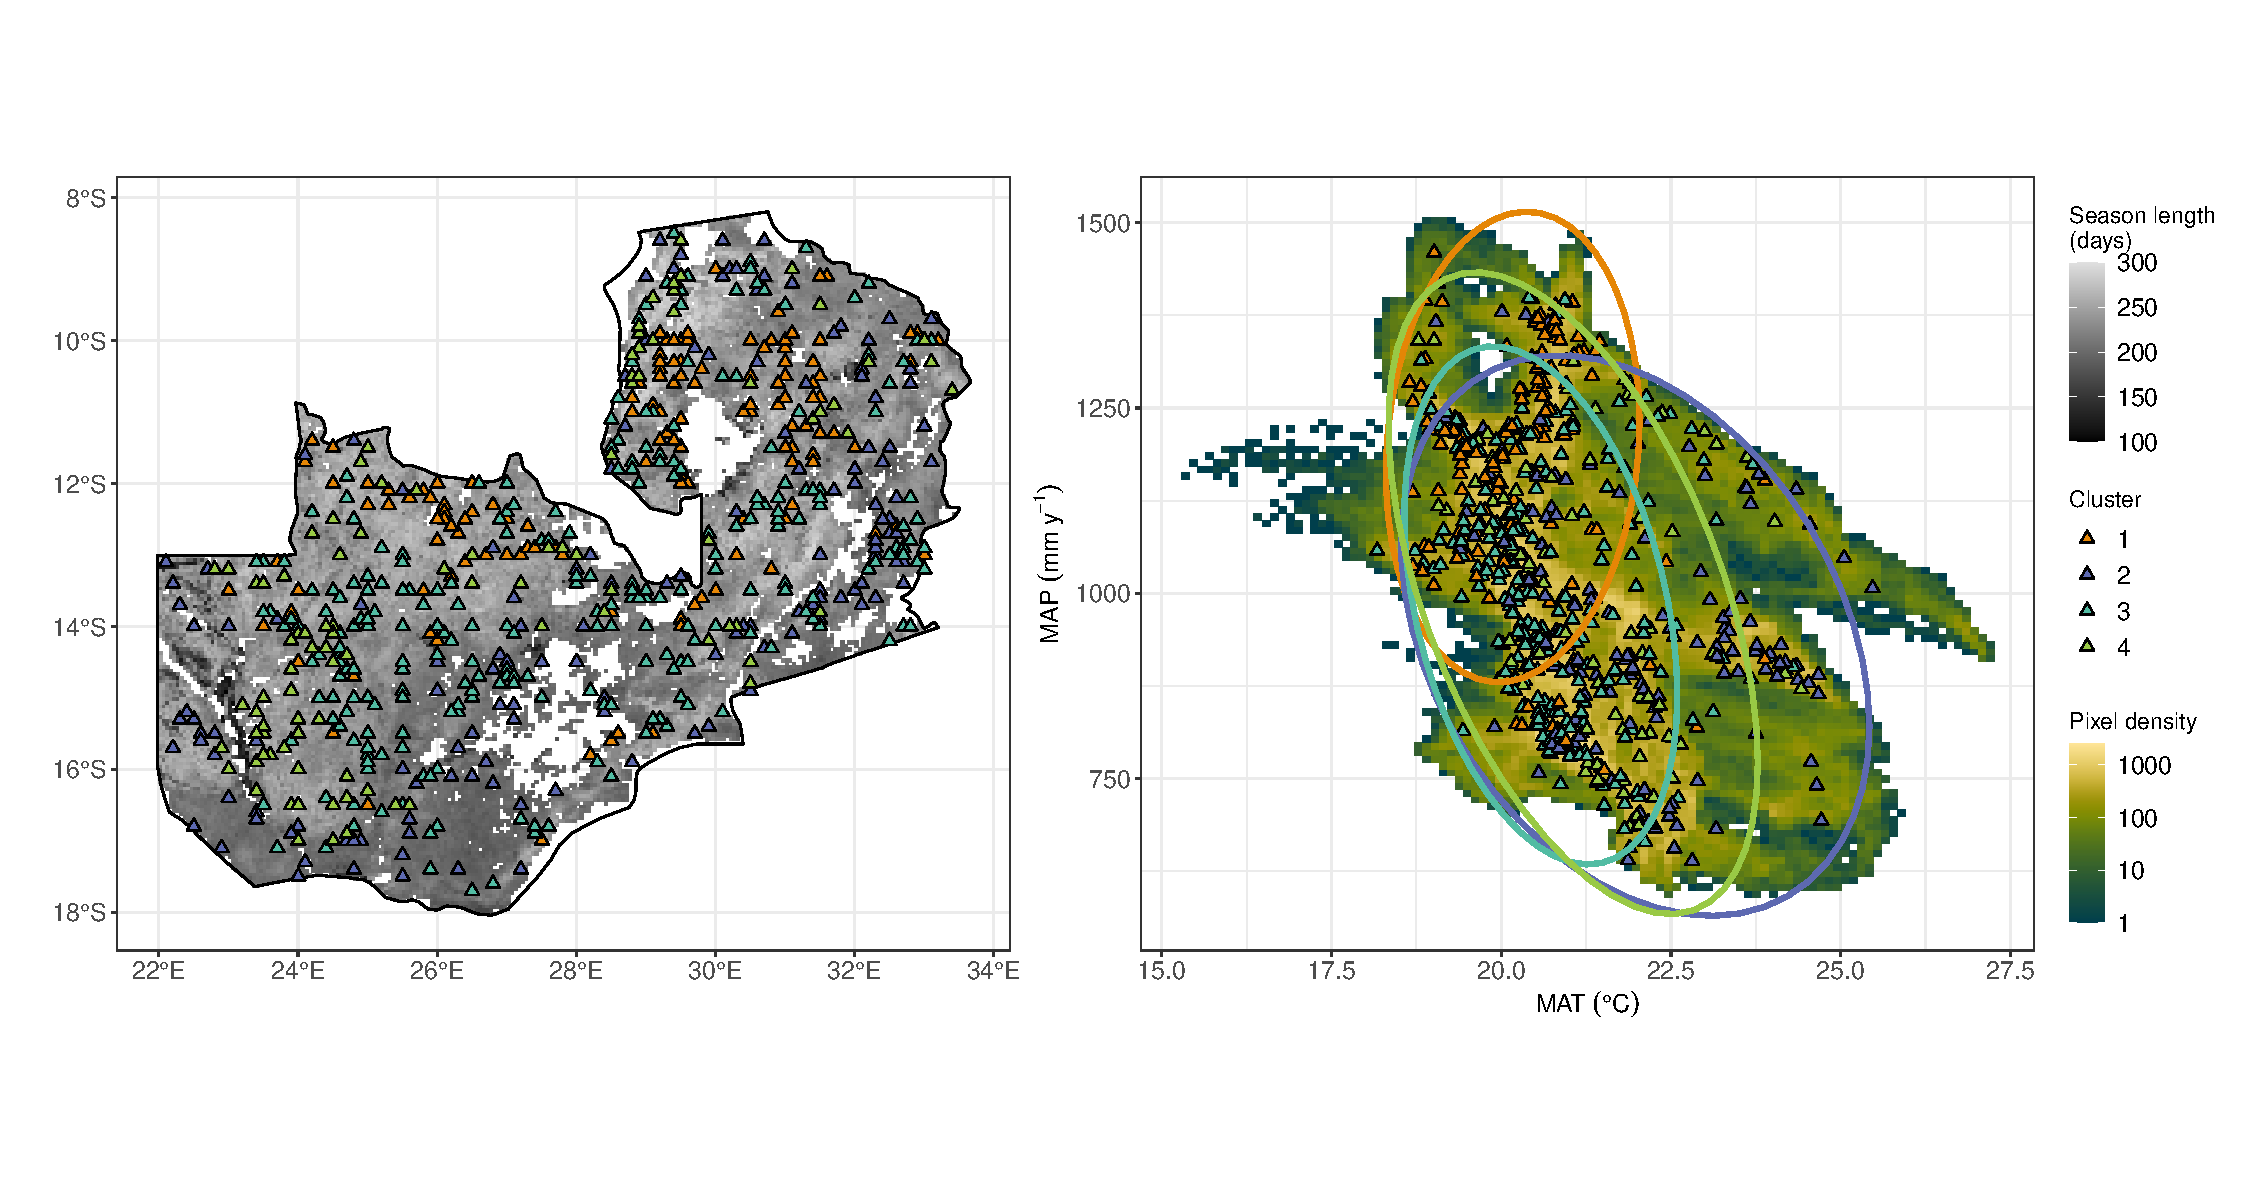
\includegraphics[width=\linewidth]{img/plot_loc_clim}
	\caption[Map of study sites in Zambia]{Distribution of study sites, within Zambia (left), and in climate space (right). Sites are shown as triangles, each consisting of four plots, coloured according to vegetation type cluster. Zambia is shaded according to growing season length, estimated by the MODIS VIPPHEN-EVI2 product, at 0.05\textdegree{} spatial resolution \citep{VIPPHEN}. The growing season length layer is masked by the MODIS MCD12Q1 land cover map from 2015 \citep{MCD12Q1}, using the International Geosphere-Biosphere Programme (IGBP) classification to remove all pixels occurring in wetlands, croplands, water bodies, and urban areas. Climate space is represented by Mean Annual Temperature (MAT) and Mean Annual Precipitation (MAP), extracted from the WorldClim dataset at 30 arc second resolution, between 1970 and 2000 \citep{Fick2017}. The shaded area in the right panel shows the climate space of Zambia, showing the density of pixels for given values of MAT and MAP. The ellipses in the right panel show the 95\% confidence interval for the climate space of each site.} 
	\label{phen:plot_loc_clim}
\end{figure}

\begin{landscape}
\begin{table}[tb] 
	\caption[Description of vegetation types]{Descriptive statistics for each of the vegetation type clusters to which each plot in the study was assigned. Numeric values of species richness, stems ha\textsuperscript{-1} and AGB represent medians and interquartile ranges (75th - 25th percentile).} 
	\label{befr:clust_summ} 
\setlength\tabcolsep{2pt}
\begin{tabular}{lS[table-format=3.2,table-column-width=0.5cm]ccc}\toprule
{Cluster} & \multicolumn{1}{p{2cm}}{\centering N\\Plots} & \multicolumn{1}{p{2cm}}{\centering Species\\Richness} & \multicolumn{1}{p{2.5cm}}{\centering Stem density\\(stems ha\textsuperscript{-1})} & \multicolumn{1}{p{2cm}}{\centering AGB\\(t ha\textsuperscript{-1})} \\
\midrule
Core miombo & 523 & 20(16.9) & 204(142.5) & 44.2(36.11) \\
ex-Acacia & 188 & 12(10.3) & 181(166.5) & 54.5(61.33) \\
Mopane & 58 & 10(10.2) & 186(125.6) & 42.7(32.83) \\ 
Baikiaea & 466 & 12(13.7) & 178(129.5) & 36.9(26.98) \\ 
\bottomrule
\end{tabular} 
\end{table} 

\end{landscape}

\begin{figure}
	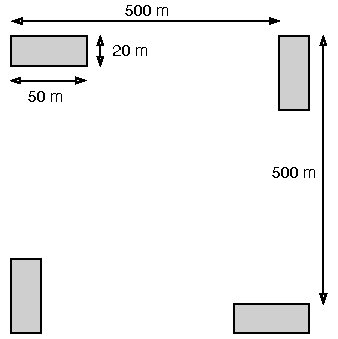
\includegraphics[width=0.5\linewidth]{img/schematic}
	\caption[Schematic diagram of plot layout within a site]{Schematic diagram of plot layout within a site. Each 20$\times$50 m (0.1 ha) plot is shaded grey. Note that the plot dimensions are not to scale.}
	\label{phen:schematic}
\end{figure}

Within each plot, the species of all trees with at least one stem $\geq$\stemSize{} cm DBH were recorded. Plot data were aggregated to the site level for analyses to avoid pseudo-replication, and to link with the more spatially coarse phenology data. Tree species composition varied little among the four plots within a site, and were treated as representative of the woodland in the local area. Using the Bray-Curtis dissimilarity index on species basal area data \citep{Faith1987}, we calculated that the mean pairwise compositional distance between plots within a site was lower than the mean compositional distance across all pairs of plots in \plotDistPer{}\% of cases.

\subsection{Plot data analysis} 
\label{phen:ssec:plot_analysis}

To classify variation in tree species composition we used agglomerative hierarchical clustering on species basal area data \citep{Kreft2010, Fayolle2014}. To guard against sensitivity to rare individuals, which can preclude meaningful cluster delineation across such a large species compositional range, we excluded species with less than five records. We used Ward's algorithm to define clusters \citep{Murtagh2014}, based on the Bray-Curtis distance between pairs of sites. We determined the optimal number of clusters by maximising the mean silhouette width among clusters \citep{Rousseeuw1987}. Vegetation type clusters were used later as interaction terms in linear models. We described the vegetation types represented by each of the clusters using a Dufr\^{e}ne-Legendre indicator species analysis \citep{Dufrene1997}. \Numberstringnum{\nCluster} vegetation type clusters were identified during hierarchical clustering. The silhouette value of the clustering algorithm reached \silBest{}. 

To describe the species diversity of each site, we calculated the Shannon-Wiener index ($H'$) from species basal area rather than individual abundance, as a measure of species diversity effectively weighted by a species' contribution to canopy occupancy and thus by contribution to the phenological signal. $H'$ was transformed to the first order numbers-equivalent ($^1\!D$) of $H'$, calculated as $e^{H'}$ \citep{Jost2007}. We use $^1\!D$ as the primary measure of species diversity in our statistical models, and is subsequently referred to as species diversity. Additionally, we calculated a separate measure of abundance evenness, using the Shannon Equitability index ($E_{H'}$) \citep{Smith1996}. $E_{H'}$ was calculated as the ratio of basal area Shannon-Wiener diversity index to the natural log of total basal area per site. To describe average tree size, we calculated the quadratic mean of stem diameters per site \citep{Curtis2000}. The quadratic mean gives more weight to large trees and is thus more appropriate for our use, where we are interested in the contribution of large trees to land-surface phenology. 

\subsection{Land-surface phenology data}
\label{phen:ssec:phen_data}

To quantify phenology at each site, we used the MODIS MOD13Q1 satellite data product at 250 m resolution \citep{MOD13Q1}. The MOD13Q1 product provides an Enhanced Vegetation Index (EVI) time series at 16 day intervals. EVI is widely used as a measure of vegetation growth and the cumulative sum of EVI is well-correlated with Gross Primary Productivity (GPP), thus providing a measure of land-surface phenology that is relevant to carbon cycling \citep{Sjostrom2011}. We used all scenes from January 2010 to December 2020 with less than 20\% cloud cover covering the study area. All sites were determined to have a single annual growing season according to the MODIS VIPPHEN product \citep{VIPPHEN}, which assigns pixels (0.05\textdegree, 5.55 km at equator) up to three growing seasons per year. We stacked yearly data between 2010 and 2020 and fit a General Additive Model (GAM) to produce an average EVI curve (\autoref{phen:ts_example}). We estimated the start and end of the growing season using first derivatives of the GAM. The start of the growing season was identified as the first day where the model slope exceeds half of the maximum positive model slope for a continuous period of \modisWin{} or more days, using only backwards looking data, following \citet{White2009}. Similarly, we defined the end of the growing season as the final day of the latest \trmmWin{} day period where the GAM slope meets or exceeds half of the maximum negative slope. We estimated the length of the growing season as the number of days between the start and end of the growing season. We calculated cumulative EVI as the area under the EVI curve during the growing season, and is reported in the results divided by \eviDiv{}, to put it on a similar scale to other variables. We estimated the green-up rate as the slope of a linear model across EVI values between the start of the growing season and the point at which the slope reduces below half of the maximum positive slope. Similarly the senescence rate was estimated as the slope of a linear model between the latest point where the slope of decrease fell below half of the maximum negative slope and the end of the growing season. We validated our calculations of cumulative EVI, mean annual EVI, growing season length, season start date, season end date, green-up rate and senescence rate with calculations made by the MODIS VIPPHEN product with linear models comparing the two datasets across our study sites (\autoref{phen:vipphen_compare}, \autoref{phen:annot_df}). We chose not to use the MODIS VIPPHEN product directly due to its more coarse spatial resolution (0.05\textdegree, 5.55 km at equator).

Precipitation data were gathered using the ``GPM IMERG Final Precipitation L3 1 day V06'' dataset, which has a pixel size of 0.1\textdegree (11.1 km at the equator) \citep{IMERG}, between 2010 and 2020. Daily total precipitation was separated into three periods: precipitation during the growing season (wet season precipitation), precipitation in the 90 day period before the onset of the growing season (pre-green-up precipitation), and precipitation in 90 day period before the onset of senescence at the end of the growing season (pre-senescence precipitation). Wet season limits were defined as for the EVI data, using the first derivative of a GAM to create a curve for each site using stacked yearly precipitation data, from which we estimated the half-maximum positive and negative slope to identify where the GAM model exceeded these slope thresholds for a consistent period of 20 days or more. Mean diurnal temperature range (Diurnal dT) was calculated as the mean of monthly temperature range from the WorldClim database, using the BioClim variables, with a pixel size of 30 arc seconds (926 m at the equator) \citep{Fick2017}, averaged across all years of available data (1970-2000). 

We calculated the lag between the onset of the growing season and the onset of the wet season as the difference between these two dates. We performed a similar calculation to estimate the lag between the end of the growing season and the end of the wet season. These two metrics are referred to as ``green-up lag'' and ``senescence lag'' hereafter. To aid interpretation, we reversed the sign of the green-up lag measurements, so that larger values indicate earlier pre-rain green-up.

\begin{figure}
	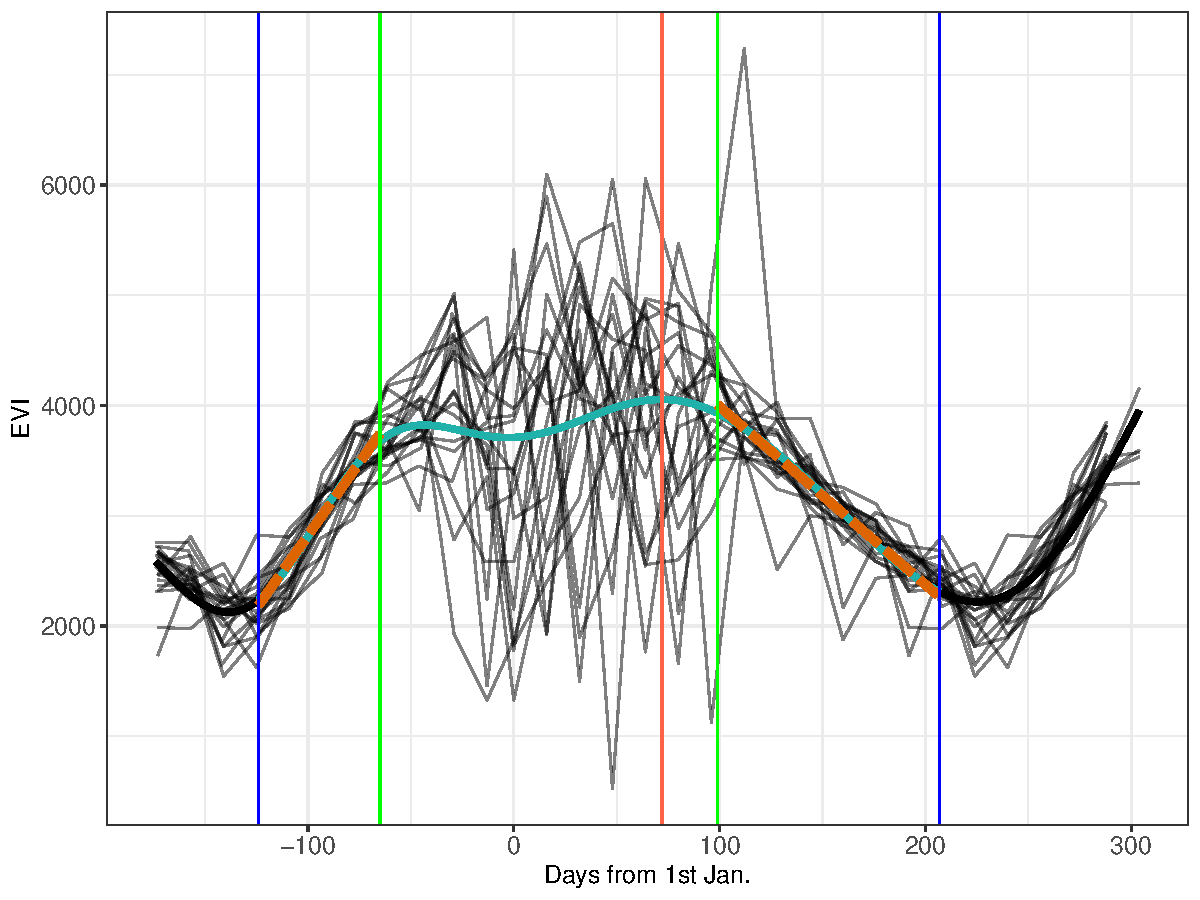
\includegraphics[width=0.8\linewidth]{img/ts_example}
	\caption[Annotated EVI time series]{Example EVI time series, demonstrating the metrics derived from it. Thin black lines show the raw EVI time series, with one line for each annual growing season. The thick cyan line shows the GAM fit. The blue vertical lines show the minima which bound the growing season. The green vertical lines show the end of the green-up period and start of the senescence period, respectively. The red vertical line shows the maximum EVI value reached within the growing season. The shaded cyan area of the GAM fit shows the growing season, as defined by the first derivative of the GAM curve. The two orange dashed lines are linear regressions predicting the green-up rate and senescence rate at the start and end of the growing season, respectively. Note that while the raw EVI time series fluctuate greatly around the middle of the growing season, mostly due to cloud cover, the GAM fit effectively smooths this variation to estimate the average EVI over the 10 years of data.}
	\label{phen:ts_example}
\end{figure}

\subsection{Statistical modelling}
\label{phen:ssec:models}

We used multivariate linear models to assess the role of tree species diversity and woodland structure on each phenological metric. We defined a maximal model structure including the explanatory variables of species diversity, evenness, and tree size alongside climatic variables shown by previous studies to strongly influence land-surface phenology. We included interaction terms of species diversity, species evenness, and tree size with vegetation type. The maximal model was compared to models with different subsets of explanatory variables, using the model log likelihood, AIC (Akaike Information Criteria), and adjusted R\textsuperscript{2} values for each model, to determine which combination of explanatory variables and their interactions with vegetation type best explained each phenological metric. Where two similar models were within 2 AIC points of each other, the model with fewer terms was chosen as the best model, to maximise model parsimony. Explanatory variables in each model were transformed to achieve normality where necessary and standardised to Z-scores prior to modelling to allow comparison of slope coefficients within a given model.

We used the \texttt{ggeffects} package to estimate the marginal means of the effects of species diversity, species evenness, and tree size on each phenological metric among vegetation types, where those terms appeared in the best model identified during model selection \citep{ggeffects}. Estimating marginal means entails generating model predictions across values of a focal variable, while holding non-focal variables constant at their reference value.

To describe variation in land-surface phenology within and among vegetation clusters we conducted a simple MANOVA using the phenological metrics as response variables, followed by post-hoc Tukey's tests between each pairwise combination of vegetation clusters per phenological metric, to test whether vegetation clusters differed significantly in their land-surface phenology. We also visually compared the mean EVI GAM fits for each cluster within the growing season. All statistical analyses were conducted in R version 4.1.0 \citep{R2020}.

\section{Results}
\label{phen:sec:results}

Our models effectively predicted cumulative EVI, season length, green-up lag, and green-up rate, while senescence lag and senescence rate were poorly constrained even in the best fitting models. Nevertheless, all models were of better quality than a naive model including only mean annual precipitation and mean annual diurnal temperature range (\autoref{phen:mod_stat}). Model selection showed that both tree species diversity and evenness were significant predictors of cumulative EVI, growing season length, and green-up lag, while senescence lag, senescence rate, and green-up rate were better explained by climate only (\autoref{phen:mod_slopes}). Despite the `best' model for senescence lag including diversity as an explanatory variable, the slope of this effect was negligible, with a wide standard error, and the model itself only explained \senesLagrsq{}\%.

As expected (H\textsubscript{1}), species diversity and wet season precipitation both had positive significant effects on cumulative EVI and growing season length. In contrast, abundance evenness, the other aspect of tree species diversity in our models, had a significant negative effect on these three phenological metrics (\autoref{phen:mod_slopes}). Similarly, species diversity increased green-up lag, i.e. the length of the period between green-up and wet season onset, while evenness caused a decrease in green-up lag (H\textsubscript{2}). The positive effect of diversity was comparable to the effects of pre-green-up precipitation and diurnal temperature range, which also increased green-up lag. The best model predicting green-up lag explained \greenLagrsq{}\% of the variance in this phenological metric.

Larger average tree size, measured by the quadratic mean of stem DBH per site, was only included and significant in the best model for senescence lag, where it caused earlier senescence with respect to the end of the wet season (H\textsubscript{5}). None of the other phenological metrics were significantly affected by average tree size. As mentioned previously however, senescence lag was poorly constrained in our models, with the best model explaining only \senesLagrsq{}\% of the variance in senescence lag.

The \numberstringnum{\nCluster} vegetation type clusters exhibited some spatial and climatic stratification (\autoref{phen:plot_loc_clim}). Cluster 1 was largely absent from the southwest of the country, occurring predominantly in higher rainfall regions to the north. Cluster 4 dominated the southwest of the country (\autoref{phen:clust_summ}). Cluster 2, consists of small stature Zambesian Combretaceae woodlands, as described by \citet{Dinerstein2017} and \citet{Chidumayo2001}, and is not dominated by the same archetypal Detarioideae canopy tree species as miombo woodland. It is possible that these woodlands represent highly disturbed miombo woodlands where large trees may have been removed by humans or by fire induced mortality. Cluster 2 occurs over a wide climatic range, and contains some of the warmest sites in the dataset. Clusters 1, 3 and 4 represent varieties of miombo woodland, dominated by \textit{Brachystegia} spp. and \textit{Julbernardia} spp., with different secondary species. Cluster 1, occurring in predominantly in the north, represents wet miombo, as defined by \citet{White1983}, while Cluster 3 represents the corresponding dry miombo. Cluster 4, possibly represents the eastern extent of the biogeographically distinct Angolan miombo woodlands, with the notable abundance of \textit{Guibourtia coleosperma} and \textit{Cryptosepalum exfoliatum} \citep{Huntley1994}. Median species richness and the range of species richness values per site is similar across all vegetation clusters (\autoref{phen:clust_summ}). 

The slope of the relationship between species diversity and phenological metrics varied among vegetation types (H\textsubscript{4}) (\autoref{phen:mod_marg}). According to post-hoc Tukey's tests on marginal effects (\autoref{phen:lsq_terms}), Cluster 2 differed from all other clusters in the effect of species diversity on cumulative EVI, growing season length, and pre-rain green-up lag. Clusters 1 and 4 appear to show no positive effect of diversity on cumulative EVI and Cluster 4 also showed a negative effect of diversity on season length. The effect of diversity and evenness on green-up lag were consistent among all vegetation types. Cluster 2 appears to show a divergent positive effect of evenness on cumulative EVI compared to the other clusters. 
 
Clusters, 1, 3 and 4 were largely similar in their density distribution of the six phenological metrics, while Cluster 2 had more plots with lower cumulative EVI and a shorter growing season (\autoref{phen:phen_dens_clust}). A MANOVA including all phenological metrics showed a significant difference among vegetation clusters (\phenManova{}). Post-hoc Tukey's tests showed significant differences between Cluster 2 and the other three clusters for all phenological metrics (\autoref{phen:tukey_terms}). Cluster 2 had a significantly shorter growing season than the other clusters, caused by both later green-up and earlier senescence. Cluster 2 also had a higher maximum EVI than the other clusters (\autoref{phen:gam_compare_clust}). The vast majority of plots, regardless of vegetation type, exhibited some degree of pre-rain green-up, and all plots exhibited some degree of senescence lag (\autoref{phen:phen_dens_clust}).


\begin{figure}
	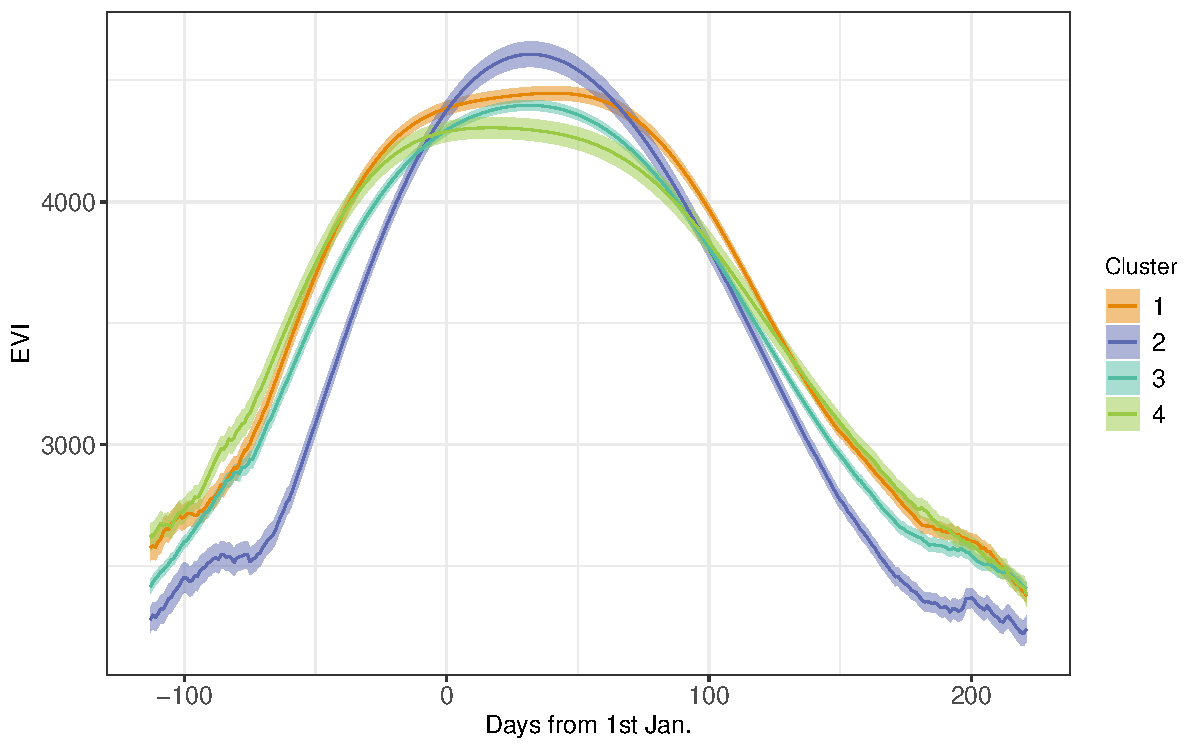
\includegraphics[width=\linewidth]{img/gam_compare_clust}
	\caption[Mean EVI GAMs per vegetation type]{Mean GAMs of EVI over the growing season for each vegetation type cluster. Shaded ribbons are 95\% confidence intervals.}
	\label{phen:gam_compare_clust}
\end{figure}

% latex table generated in R 4.1.0 by xtable 1.8-4 package
% Fri Jul 23 16:11:32 2021
\begin{table}[H]
\centering
\begin{tabular}{rccc}
  \hline
Response & $\delta$AIC & R\textsuperscript{2}\textsubscript{adj} & $\delta$logLik \\ 
  \hline
Cumulative EVI & 74.8 & 0.34 & -52.38 \\ 
  Season length & 75.3 & 0.20 & -52.63 \\ 
  Green-up rate & 48.2 & 0.21 & -39.09 \\ 
  Senescence rate & 83.2 & 0.15 & -56.59 \\ 
  Green-up lag & 100.3 & 0.33 & -65.15 \\ 
  Senescence lag & 21.3 & 0.11 & -25.64 \\ 
   \hline
\end{tabular}
\caption{Model fit statistics for the best model describing each phenological metric.} 
\label{mod_stat}
\end{table}

 

\begin{figure}
	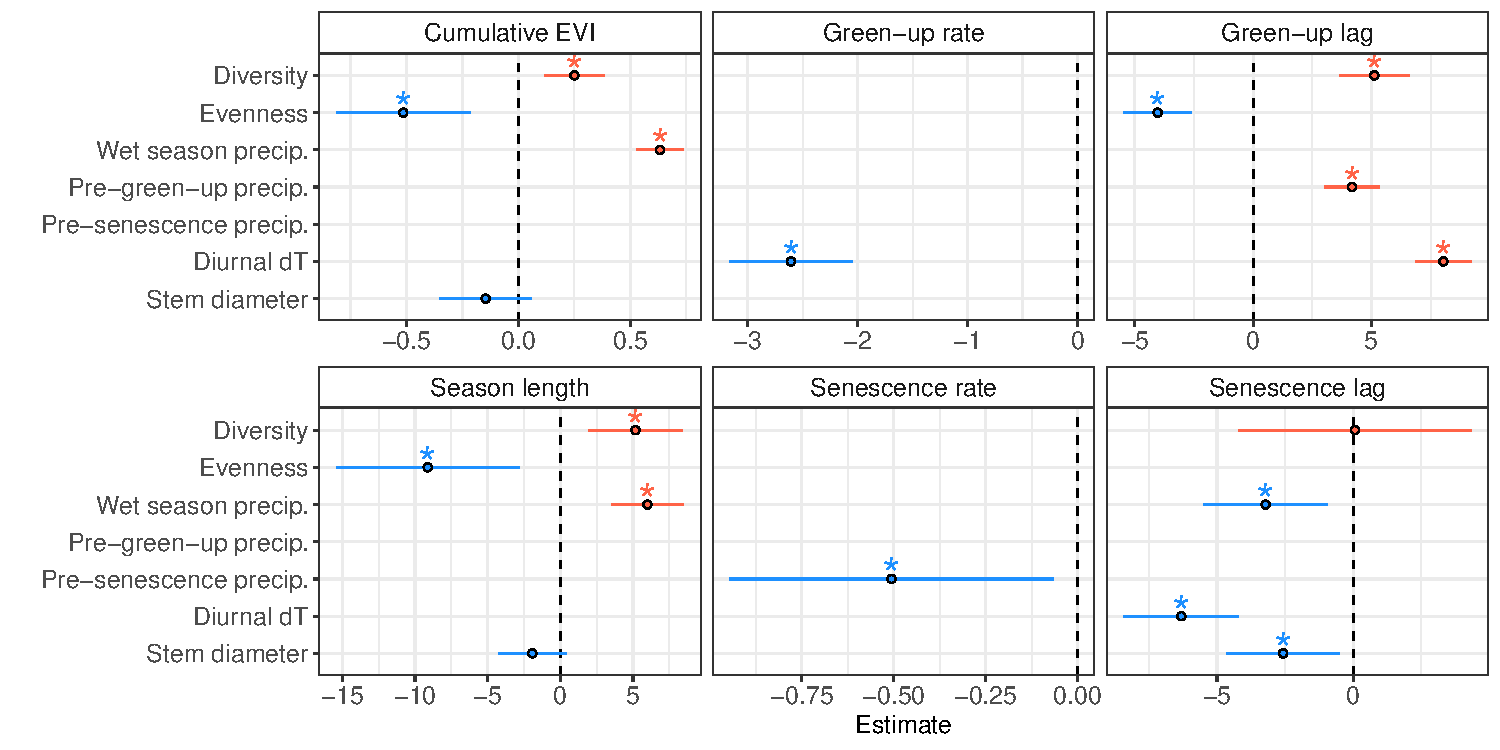
\includegraphics[width=\linewidth]{img/mod_slopes}
	\caption[Model slope coefficients for each phenological metric]{Standardised slope coefficients for each best model of a phenological metric. Slope estimates are $\pm$1 standard error. Slope estimates where the interval does not overlap zero are considered to be significant effects and are marked by asterisks.}
	\label{phen:mod_slopes}
\end{figure}

\begin{figure}
	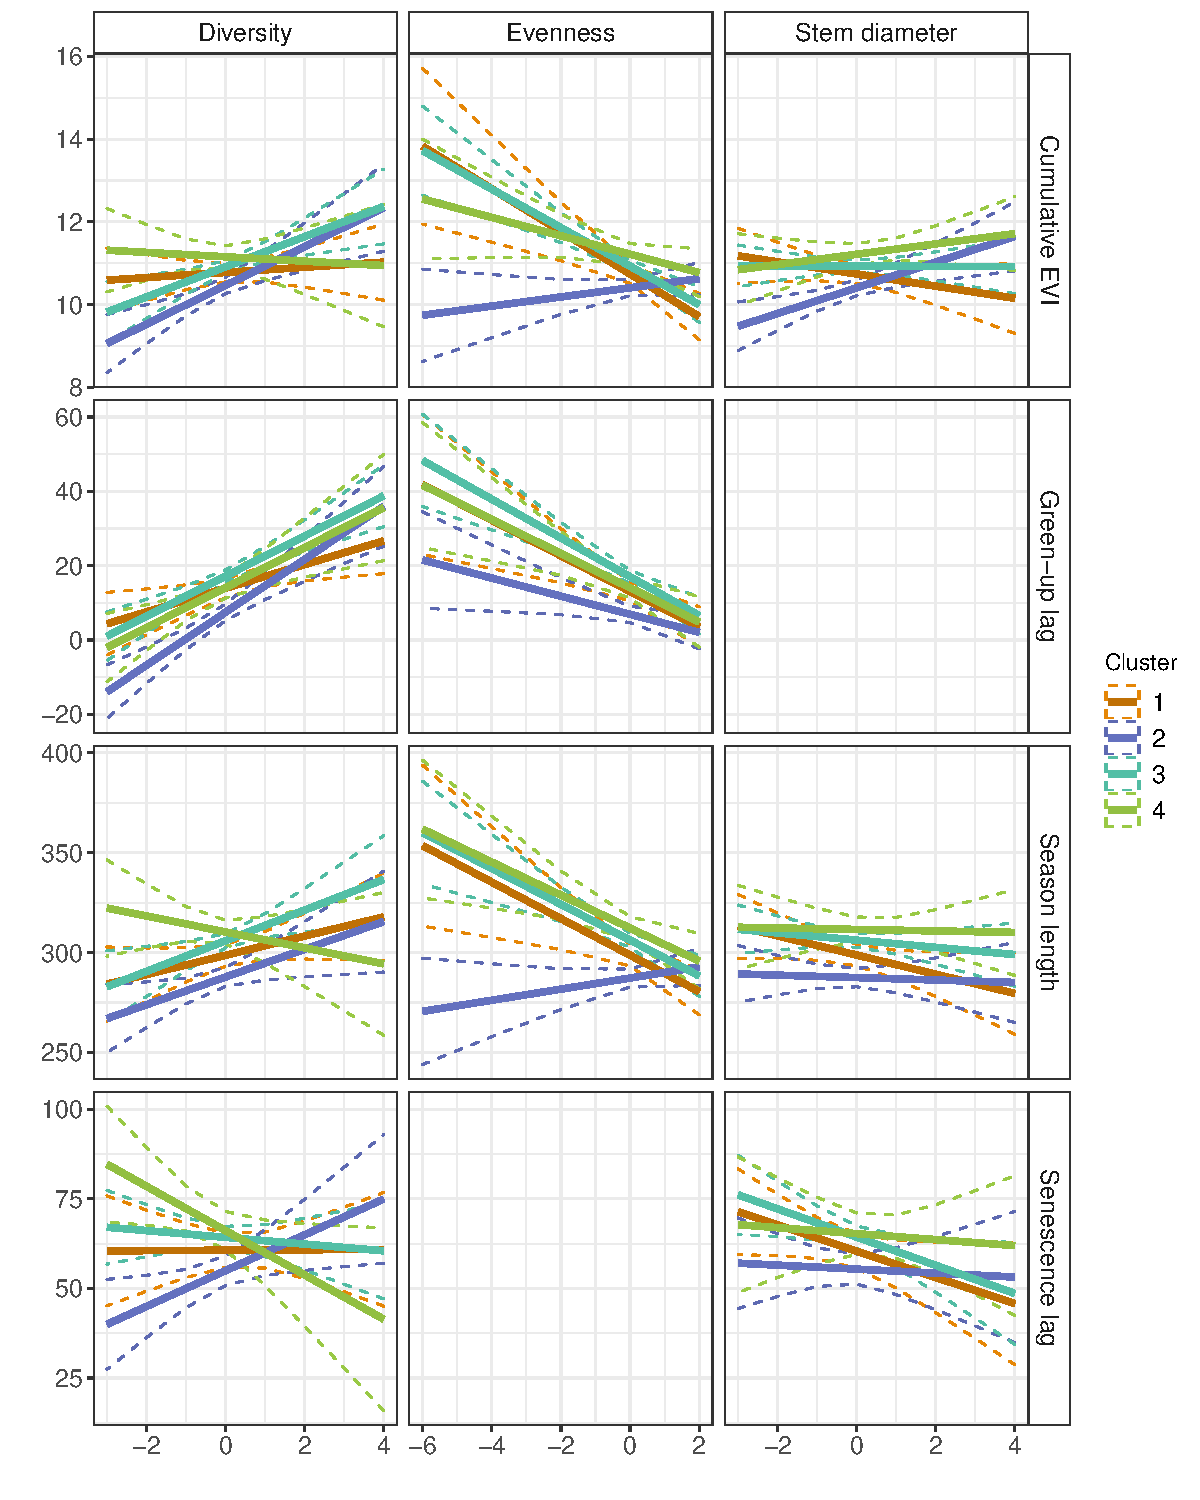
\includegraphics[width=\linewidth]{img/mod_marg}
	\caption[Marginal effects of species diversity on each phenological metric per vegetation type]{Marginal effects of tree species diversity, evenness, and tree size on each of the phenological metrics, using the maximal mixed effects model, for each vegetation cluster. Dotted lines represent 95\% confidence intervals.}
	\label{phen:mod_marg}
\end{figure}

\begin{figure}
	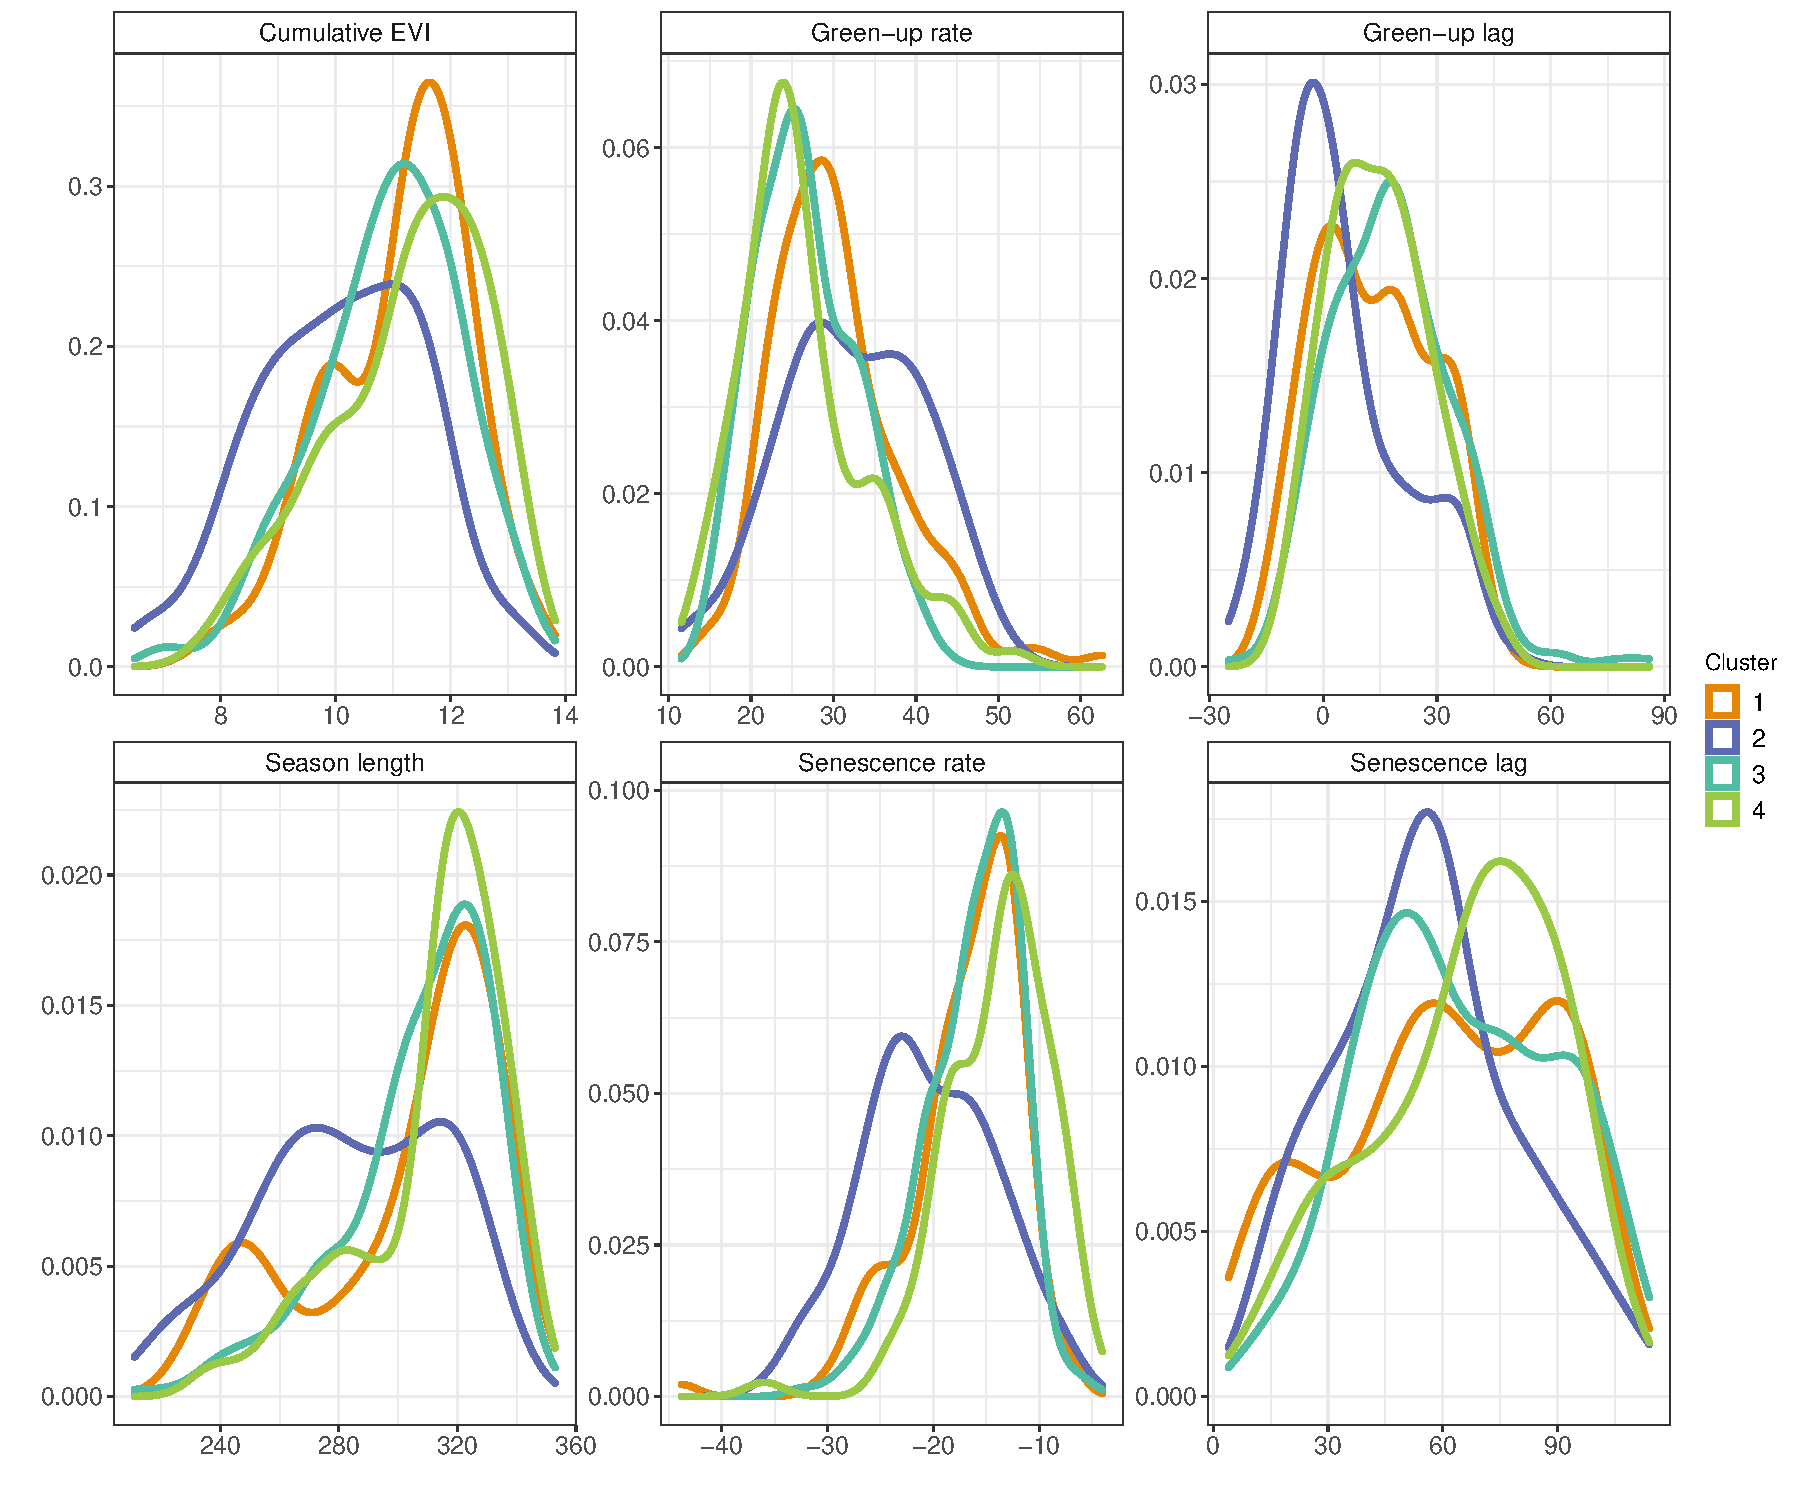
\includegraphics[width=\linewidth]{img/phen_dens_clust}
	\caption[Density distribution of phenological metrics per vegetation type]{Density distribution of the six phenological metrics used in the study, grouped by vegetation cluster.}
	\label{phen:phen_dens_clust}
\end{figure}

\section{Discussion}
\label{phen:sec:discussion}

In this study we have demonstrated clear and measurable effects of tree species diversity, evenness, and composition on various aspects of land-surface phenology in Zambian deciduous savannas, independent of the effects of climatic variation. We showed that tree species diversity led to an increase in cumulative EVI and growing season length in certain vegetation types. Additionally, species diversity caused the onset of greening to occur earlier with respect to the start of the wet season, in all vegetation types. Our study lends support for a positive biodiversity-ecosystem function relationship in deciduous savannas, operating through its influence on land-surface phenology, with a longer growing season and greater cumulative EVI suggesting greater primary productivity in species rich woodlands. Additionally, our finding that species diversity causes earlier pre-rain green-up suggests that diverse woodlands are more resilient to varying precipitation patterns, by producing foliage in advance of seasonal rainfall. This provides early forage for herbivores \citep{Morellato2016}, and provides facilitative effects such as cover and hydraulic lift which benefit understorey plants \citep{Domec2010, Yu2015}. Our results highlight the role of tree species diversity as a driver of key ecosystem processes, which affect ecosystem structure, the wildlife provisioning role, and gross primary productivity.

Our finding that species diversity strongly affects patterns of land-surface phenology in deciduous Zambian woodlands provides earth surface system modellers with a means to better understand how future changes in species diversity and composition will affect land-surface phenology and therefore the carbon cycle. Incorporating predictions of biotic change into carbon cycling models has been limited \citep{Ahlstrom2015, Bodegom2011}, owing to large uncertainties in the effects of diversity on Gross Primary Productivity (GPP). Our study provides a link by demonstrating a strong positive relationship between species diversity and cumulative EVI, which itself correlates with GPP \citep{Sjostrom2011}.

While species diversity is a common measure of biodiversity, abundance evenness constitutes a second key related axis \citep{Wilsey2005, Hillebrand2008, Jost2010}. In this study, we found contrasting effects of diversity and evenness on cumulative EVI, growing season length and green-up lag. Evenness caused a decrease in these phenological metrics in miombo woodland vegetation, contrary to our hypothesis. It is possible that the negative effect of abundance evenness occurred because an increase in evenness is associated with a reduction in the dominance of a few large canopy-forming tree species (e.g. \textit{Brachystegia} spp. and \textit{Julbernardia paniculata}). Large canopy tree species have access to groundwater for a longer part of the year, due to their deep root systems and conservative growth patterns, allowing them to green-up in advance of seasonal rains and remain resilient to mid-season fluctuations in water availability \citep{Zhou2020}. Indeed, our study found that plots with larger trees tend to senesce later with respect to the end of the wet season. We found that while the three miombo vegetation types showed a negative effect of evenness on cumulative EVI and season length, Cluster 2, which was not dominated by miombo canopy tree species, showed a positive effect of evenness on these phenological metrics. 

The effect of species diversity on cumulative EVI and growing season length was driven largely by the response of vegetation Clusters 2 and 3. Cluster 2 consisted of shorter stature non-miombo vegetation. Clusters 1, and 4, which consisted of miombo vegetation, exhibited negligible species diversity effects on these two phenological metrics. However, Cluster 3, the remaining miombo vegetation type also showed a positive effect of evenness on cumulative EVI. Cluster 3 had lower annual precipitation than the other two miombo clusters, with a precipitation regime closer to that of Cluster 2, representing the dry miombo vegetation type identified by \citet{White1983}. In high precipitation miombo vegetation, it appears that the dominant archetypal miombo tree species can grow to large canopy forming trees, and that these individuals determine cumulative EVI as a result. Meanwhile, in the drier woodlands represented by Clusters 2 and 3, a genuine species diversity effect driven by niche complementarity exists. We suggest that in these drier woodlands, higher species diversity provides ecosystem level resilience to drought by increasing the breadth of water use strategies. 

Patterns of senescence were poorly predicted by species diversity and evenness in our models. \citet{Cho2017} found that tree cover, measured by MODIS LAI data, had a significant negative effect on senescence rates in savannas in South Africa, which have similar climatic conditions to the sites in our study. In most savannas, including sparse savannas, while the onset of the growing season is often driven by tree photosynthetic activity, which may precede the onset of precipitation, the end of the growing season is conversely driven by the understorey grass layer, which itself can be dependent on tree cover \citep{Cho2017, Guan2014}. Grass activity is more reactive to short-term changes in soil moisture than tree activity, and may oscillate within the senescence period \citep{Archibald2007}. This may explain the lack of a strong precipitation signal for senescence lag and senescence rate in our models. Our finding that sites with larger trees may prolong the growing season beyond the end of the rainy season corroborates these earlier studies. As average tree stem size increases, tree cover is also likely to increase \citep{Panzou2020}, reducing the relative contribution of the understorey grass layer to land-surface phenology and producing a more consistent decline in EVI during the senescence period. 

Other studies both globally and within southern African savannas have largely ignored patterns of senescence, instead focussing patterns of green-up \citep{Gallinat2015}. Most commonly, these studies simply correlate the decline of rainfall with senescence \citep{Guan2014}, but our best model suggests that diurnal temperature range is a stronger determinant of the end of the growing season than precipitation. Diurnal temperature range effectively measures mean daily temperature variability. We suggest that diurnal temperature fluctuations, particularly minimum night time temperatures, may provide cues for senescence toward the end of the wet season. In temperate ecosystems which experience autumn senescence, lower night time temperatures have been shown to increase the rate of senescence \citep{Michelson2017, Escamilla2020}, thus leaves remain green for longer when the diurnal temperature range is smaller. Similarly, our models showed that larger diurnal temperature range caused earlier pre-rain green-up, and possibly acts as a cue to initiate the growing season as well.

Alternatively, \citet{Zani2020} suggests that in resource limited environments, senescence times may largely be set by the preceding photosynthetic activity and sink-limitations on growth. For example, limited nutrient supply may prohibit photosynthesis late in the season if the preceding photosynthetic activity has depleted that supply. \citet{Reich1992} suggested that there are many direct constraints on leaf life-span such as drought and herbivory, especially in the dry tropics, which would lead to timing of senescence being set largely by the time of bud-burst. Our study corroborates this theory, showing that precipitation across the entire wet season was a better predictor of senescence lag than pre-senescence precipitation, while pre-senescence precipitation does cause variation in the rate of senescence. However, we did not find a strong correlation between green-up lag and senescence lag (\autoref{phen:phen_bivar}).

While leaf senescence may not be as important for the survival of browsing herbivores as the green-up period, the timing of senescence with respect to temperature and precipitation has important consequences for the savanna understorey microclimate. The longer leaf material remains in the canopy after the end of the wet season, the greater the microclimatic buffer for herbaceous understorey plants and animals, which require water and protection from high levels of insolation and dry air which can prevail rapidly after the end of the wet season \citep{Guan2014}. Our study merely demonstrates that more work needs to be done to properly characterise the drivers of senescence in this biome, which were poorly constrained in our models.

Our coverage of very short growing season lengths in Zambia was restricted, with a notable absence of available plot data in the northeast of the country around E30.5\textdegree{}, S11.5\textdegree{}, and E23.0\textdegree{}, S15.0\textdegree{}. These regions are largely seasonally water-logged floodplain and swampland \citep{White1983, Dinerstein2017}, and were likely excluded by the ILUA-II assessment for this reason. This also explains their divergent phenological patterns as observed in the MODIS EVI data (\autoref{phen:plot_loc_clim}). The plot data does however, provide representative coverage of growing season lengths in wooded ecosystems. While our study focusses on woodlands, the phenological behaviour of these other vegetation types should also be considered in future studies, as these may be even more sensitive to changes in climate \citep{Dean2018} and under greater land-use change pressures \citep{Langan2018}.

It is important to note that the remotely sensed EVI data used here do not only measure trees, they represent the landscape as a single unit. Nevertheless, seasonal patterns of tree leaf phenology in southern African deciduous woodlands, particularly the pre-rain green-up phenomenon, is driven almost exclusively by trees, while grass phenology tends to follow patterns of precipitation more closely \citep{Whitecross2017, Archibald2007, Higgins2011}. Grasses make a significant contribution to savanna gross primary productivity \citep{Lloyd2008}, and it was therefore in our interests to include their response in our analysis as we seek to demonstrate how tree species diversity can affect cycles of carbon exchange. Additionally, the micro-climatic effects of tree leaf canopy coverage and hydraulic lift through tree deep root systems will benefit the productivity of grasses as well as understorey tree individuals.

\section{Conclusion}
\label{phen:sec:conclusion}

Here we explored how tree species diversity, composition and woodland structure influence land surface phenology across Zambia. We showed that species diversity clearly causes earlier pre-rain green-up, across all vegetation types studied here. The length of the growing season, and ultimately woodland productivity as measured by cumulative EVI, appeared to increase with species diversity in drier woodlands only, while wetter miombo woodlands were dominated by a few canopy-forming archetypal miombo Detarioideae species regardless of species diversity. Interestingly, species evenness had a consistently negative effect on green-up lag, suggesting that pre-rain green-up is driven by canopy-forming Detarioideae species when they are dominant. Finally, we have demonstrated variation in phenological patterns among vegetation types within Zambia that are commonly not distinguished in earth system models. Our results have a range of consequences for earth system modellers as well as conservation managers working in Zambia and across the dry tropics, and lend further support to an already well established corpus of study demonstrating the positive effect of species diversity on ecosystem function.

\newpage{}
\FloatBarrier{}
\begingroup
\setstretch{1.0}
\printbibliography[heading=subbibintoc]
\endgroup

\section{Supplementary material}
\label{phen:sec:supp}
\begin{supplement} 

\begin{figure}[H]
	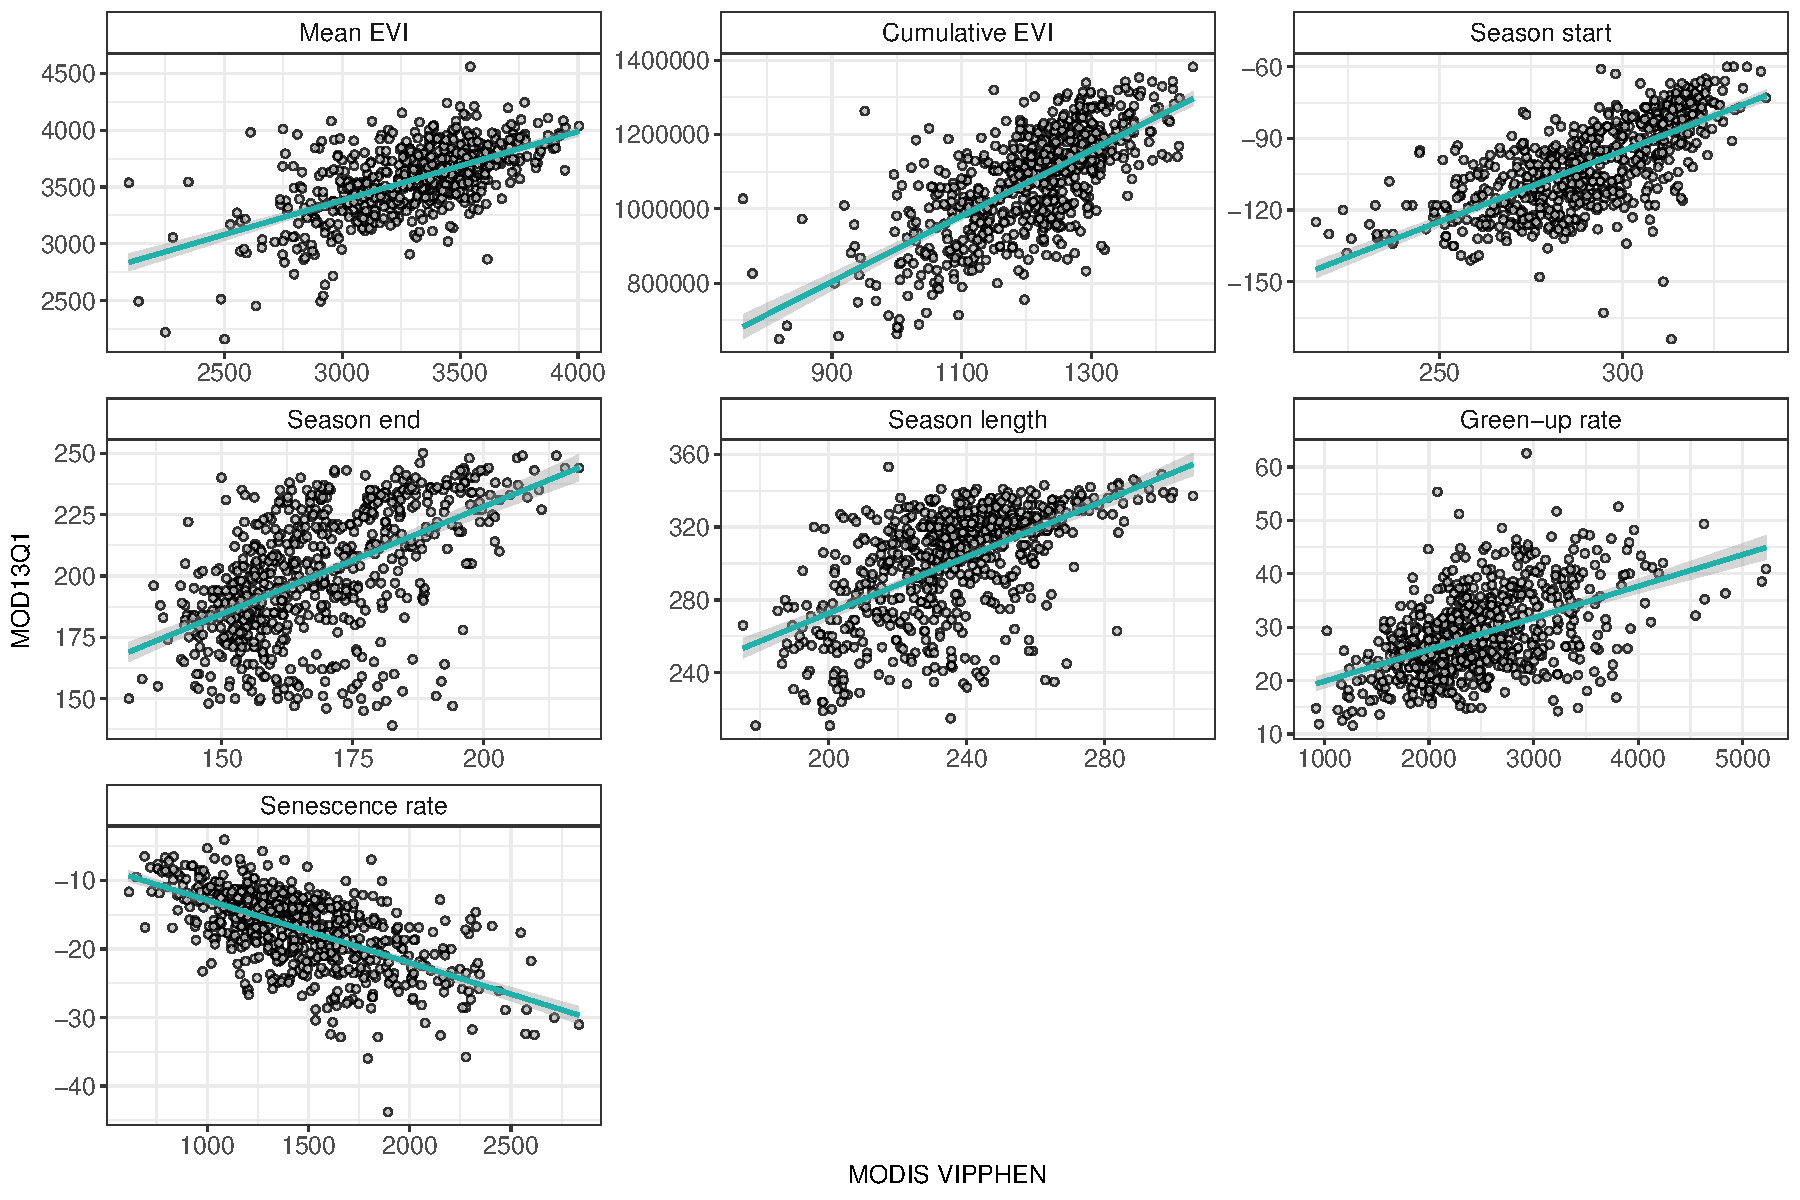
\includegraphics[width=\linewidth]{img/vipphen_compare}
	\caption[Scatter plots comparing MOD13Q1 and MODIS VIPPHEN phenological measurements]{Scatter plots showing a comparison of phenological metrics from the MODIS VIPPHEN product \citep{VIPPHEN} and those extracted from the MOD13Q1 data \citep{MOD13Q1}, for each of the sites in our study. The cyan line shows a linear model of the data, with a 95\% confidence interval.}
	\label{phen:vipphen_compare}
\end{figure}

% latex table generated in R 4.1.0 by xtable 1.8-4 package
% Fri Jul 23 16:05:31 2021
\begin{table}[h]
\caption[Model fit statistics comparing MODIS VIPPHEN and MOD13Q1 phenological metrics]{Model fit statistics for comparison of MODIS VIPPHEN and MOD13Q1 products across each of our study sites.} 
\label{phen:annot_df}
\begin{tabular}{lS[table-format=3.0]S[table-format=3.1]S[table-format=1.2]S[table-format=<1.2]}
  \toprule
{Response} & {DoF} & {F} & {R\textsuperscript{2}} & {Prob.} \\ 
  \midrule
Mean EVI & 672 & 387.0 & 0.37 & <0.05 \\ 
  Cumulative EVI & 672 & 592.6 & 0.47 & <0.05 \\ 
  Season start & 672 & 660.3 & 0.50 & <0.05 \\ 
  Season end & 672 & 285.0 & 0.30 & <0.05 \\ 
  Season length & 672 & 325.0 & 0.33 & <0.05 \\ 
  Green-up rate & 672 & 217.2 & 0.24 & <0.05 \\ 
  Senescence rate & 672 & 412.3 & 0.38 & <0.05 \\ 
   \bottomrule
\end{tabular}
\end{table}



\begin{figure}[H]
	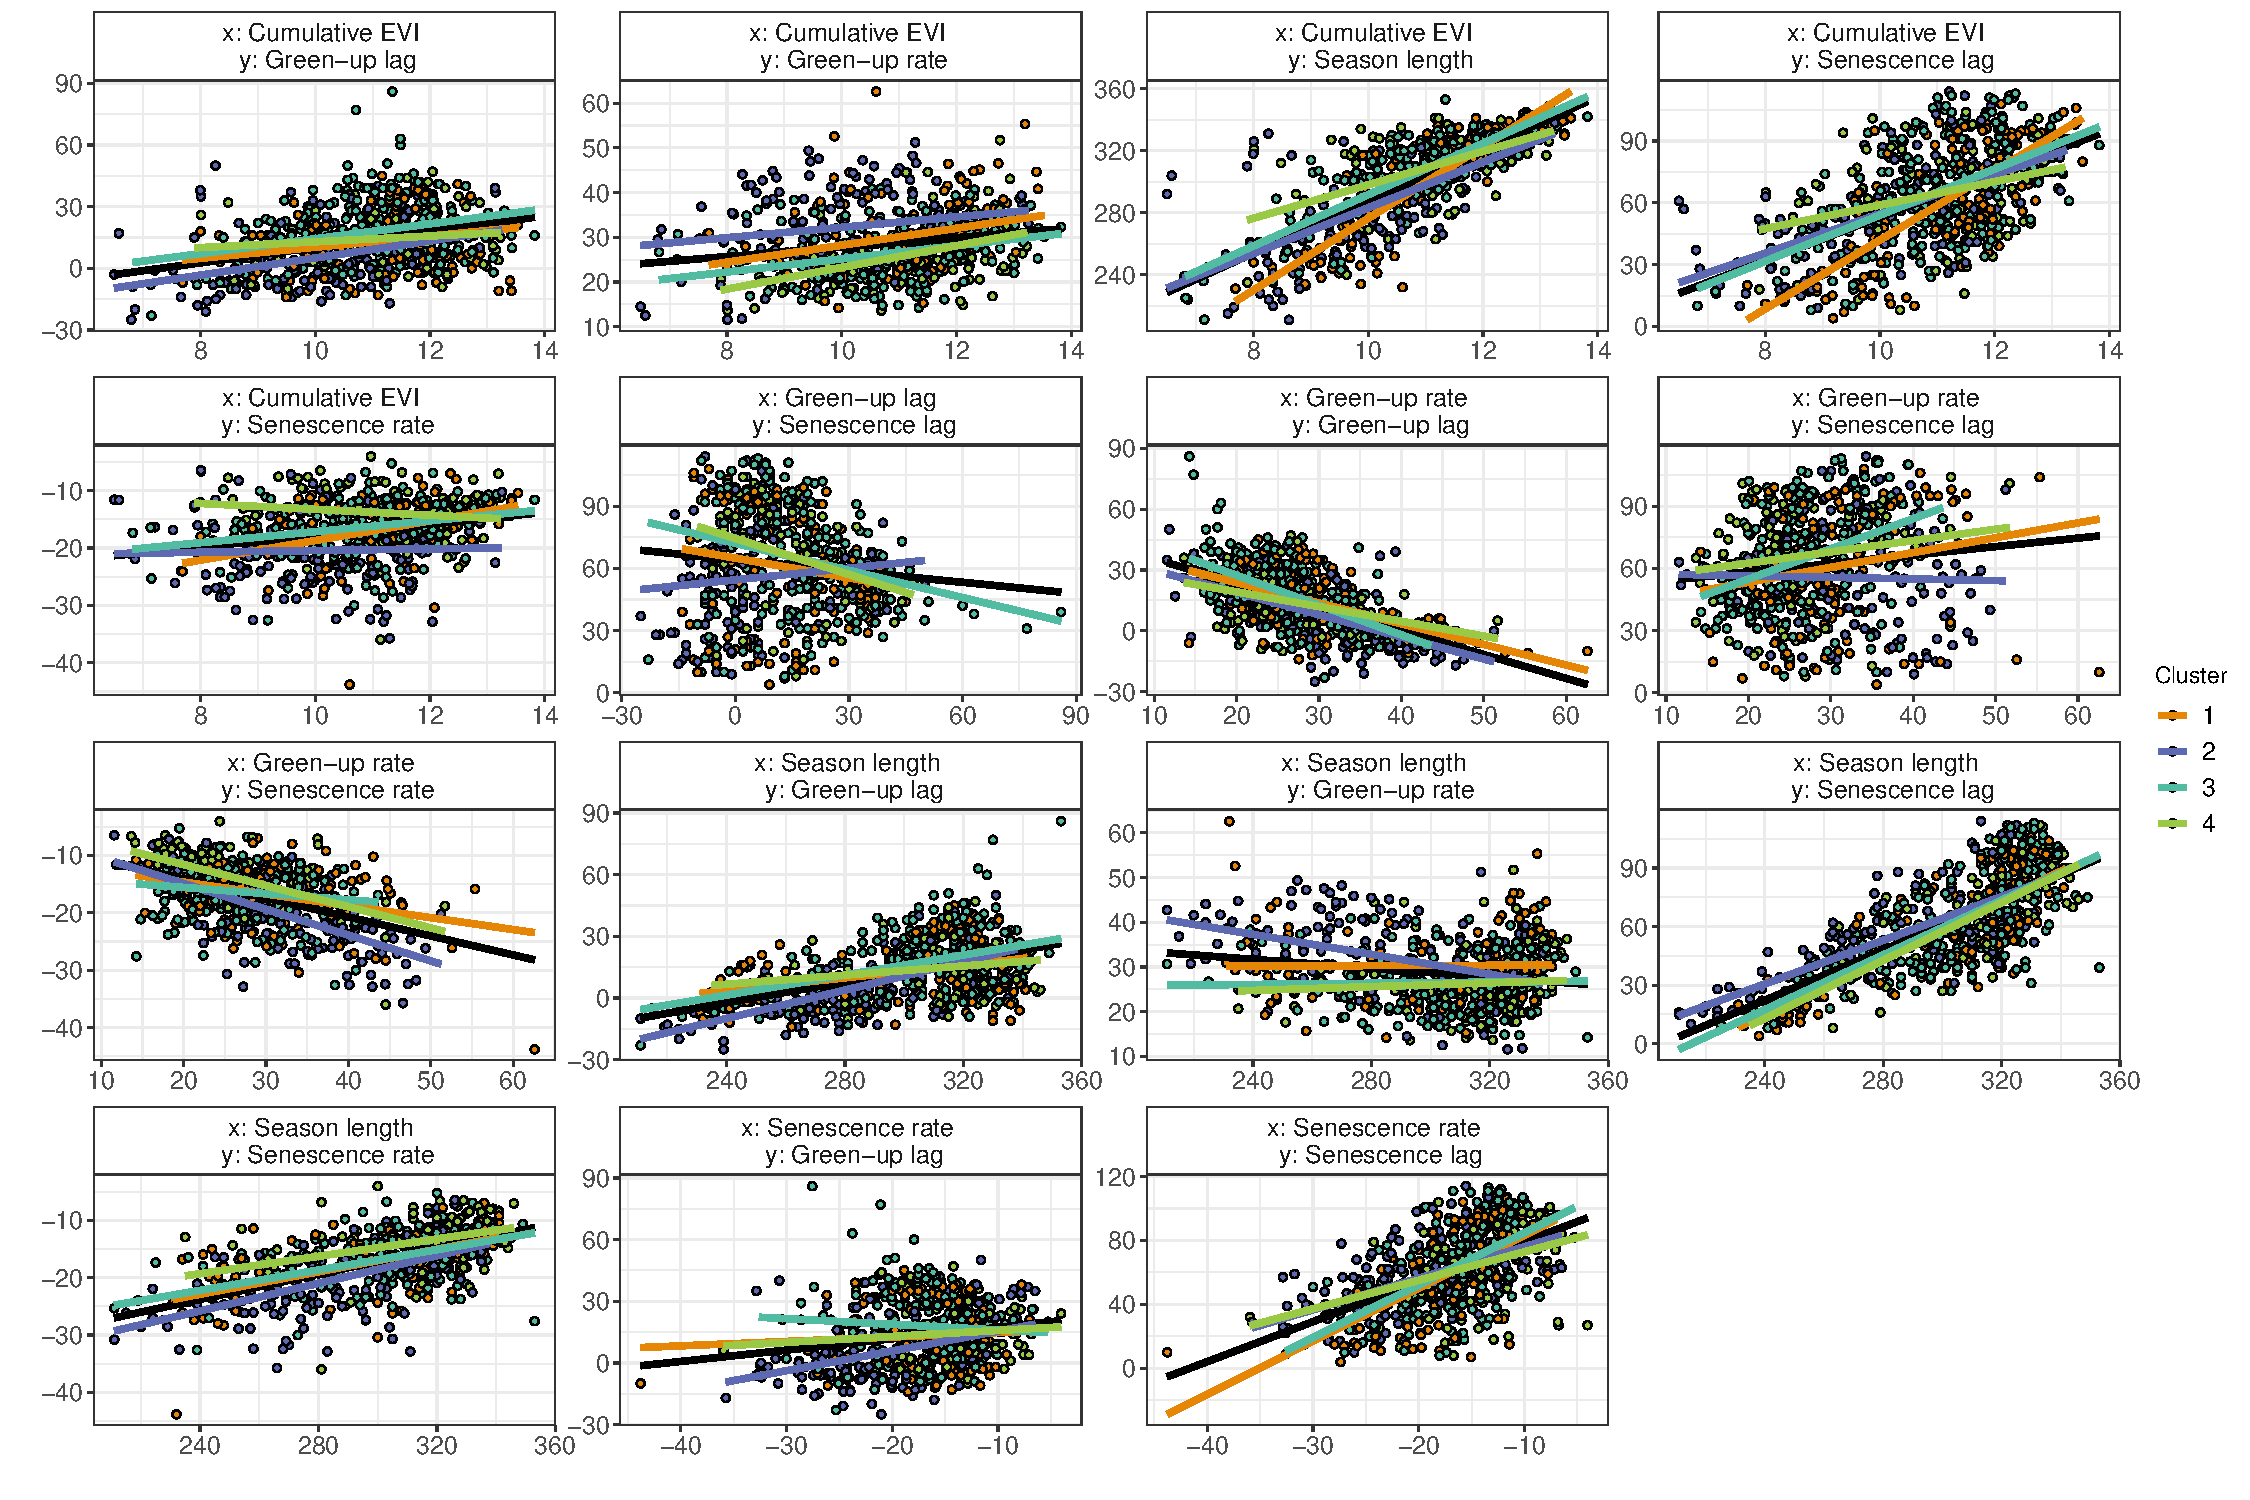
\includegraphics[width=\linewidth]{img/phen_bivar}
	\caption[Bivariate comparison of phenological metrics]{Scatter plots showing pairwise comparisons of the six phenological metrics used in this study, extracted from the MODIS MOD13Q1 product \citep{MOD13Q1}. Points represent study sites and are coloured by vegetation cluster. Linear regression line of best fit for all sites is shown as a black line, while linear regressions are shown for each vegetation cluster as coloured lines.}
	\label{phen:phen_bivar}
\end{figure}

\setlength\tabcolsep{2pt} 
% latex table generated in R 4.1.0 by xtable 1.8-4 package
% Fri Jul 23 16:11:32 2021
\begin{table}[H]
\centering
\begin{tabular}{ccccccccrrrr}
  \hline
Rank & Cluster & Precipitation & Stem diameter & Diurnal dT & Richness & Evenness & DoF & logLik & AIC & $\Delta{}$ & $W_{i}$ \\ 
  \hline
\underline{\textbf{1}} & \underline{\textbf{\checkmark}} & \underline{\textbf{\checkmark}} & \underline{\textbf{\checkmark+}} & \underline{\textbf{\checkmark}} & \underline{\textbf{\checkmark+}} & \underline{\textbf{\checkmark+}} & \underline{\textbf{19}} & \underline{\textbf{-932}} & \underline{\textbf{1903}} & \underline{\textbf{0}} & \underline{\textbf{0.380}} \\ 
  2 & \checkmark & \checkmark & \checkmark+ &  & \checkmark+ & \checkmark+ & 18 & -933 & 1903 & 0 & 0.366 \\ 
  3 & \checkmark & \checkmark & \checkmark+ & \checkmark & \checkmark & \checkmark+ & 16 & -937 & 1906 & 4 & 0.065 \\ 
  4 & \checkmark & \checkmark & \checkmark+ &  & \checkmark & \checkmark+ & 15 & -938 & 1907 & 4 & 0.048 \\ 
  5 & \checkmark & \checkmark & \checkmark & \checkmark & \checkmark+ & \checkmark+ & 16 & -938 & 1907 & 5 & 0.040 \\ 
  6 & \checkmark & \checkmark & \checkmark &  & \checkmark+ & \checkmark+ & 15 & -939 & 1908 & 5 & 0.027 \\ 
  7 & \checkmark & \checkmark &  &  & \checkmark+ & \checkmark+ & 14 & -940 & 1908 & 6 & 0.022 \\ 
  8 & \checkmark & \checkmark &  & \checkmark & \checkmark+ & \checkmark+ & 15 & -939 & 1909 & 6 & 0.018 \\ 
  9 & \checkmark & \checkmark & \checkmark & \checkmark & \checkmark & \checkmark+ & 13 & -942 & 1910 & 8 & 0.008 \\ 
  10 & \checkmark & \checkmark & \checkmark+ &  & \checkmark+ & \checkmark & 15 & -941 & 1911 & 9 & 0.005 \\ 
   \hline
\end{tabular}
\caption{Cumulative EVI model selection candidate models, with fit statistics. The overall best model is marked by bold text, according to AIC and model parsimony.} 
\label{mod_sel_cum_vi}
\end{table}

% latex table generated in R 4.1.0 by xtable 1.8-4 package
% Fri Jul 23 16:11:32 2021
\begin{table}[H]
\centering
\begin{tabular}{ccccccccrrrr}
  \hline
Rank & Cluster & Precipitation & Stem diameter & Diurnal dT & Richness & Evenness & DoF & logLik & AIC & $\Delta{}$ & $W_{i}$ \\ 
  \hline
1 & \checkmark & \checkmark & \checkmark & \checkmark & \checkmark+ & \checkmark+ & 16 & -2898 & 5829 & 0 & 0.198 \\ 
  \underline{\textbf{2}} & \underline{\textbf{\checkmark}} & \underline{\textbf{\checkmark}} & \underline{\textbf{\checkmark}} & \underline{\textbf{\checkmark}} & \underline{\textbf{\checkmark}} & \underline{\textbf{\checkmark+}} & \underline{\textbf{13}} & \underline{\textbf{-2901}} & \underline{\textbf{5829}} & \underline{\textbf{0}} & \underline{\textbf{0.187}} \\ 
  3 & \checkmark & \checkmark & \checkmark &  & \checkmark+ & \checkmark+ & 15 & -2900 & 5830 & 1 & 0.106 \\ 
  4 & \checkmark & \checkmark & \checkmark &  & \checkmark & \checkmark+ & 12 & -2903 & 5830 & 1 & 0.097 \\ 
  5 & \checkmark & \checkmark &  &  & \checkmark+ & \checkmark+ & 14 & -2901 & 5830 & 2 & 0.077 \\ 
  6 & \checkmark & \checkmark &  & \checkmark & \checkmark+ & \checkmark+ & 15 & -2900 & 5831 & 2 & 0.074 \\ 
  7 & \checkmark & \checkmark &  &  & \checkmark & \checkmark+ & 11 & -2904 & 5831 & 2 & 0.068 \\ 
  8 & \checkmark & \checkmark &  & \checkmark & \checkmark & \checkmark+ & 12 & -2903 & 5831 & 2 & 0.064 \\ 
  9 & \checkmark & \checkmark & \checkmark+ & \checkmark & \checkmark+ & \checkmark+ & 19 & -2897 & 5832 & 3 & 0.036 \\ 
  10 & \checkmark & \checkmark & \checkmark+ & \checkmark & \checkmark & \checkmark+ & 16 & -2900 & 5832 & 3 & 0.034 \\ 
   \hline
\end{tabular}
\caption{Season length model selection candidate models, with fit statistics. The overall best model is marked by bold text, according to AIC and model parsimony.} 
\label{mod_sel_s1_length}
\end{table}

% latex table generated in R 4.1.0 by xtable 1.8-4 package
% Fri Jul 23 16:11:32 2021
\begin{table}[H]
\centering
\begin{tabular}{ccccccccrrrr}
  \hline
Rank & Cluster & Precipitation & Stem diameter & Diurnal dT & Richness & Evenness & DoF & logLik & AIC & $\Delta{}$ & $W_{i}$ \\ 
  \hline
\underline{\textbf{1}} & \underline{\textbf{\checkmark}} & \underline{\textbf{}} & \underline{\textbf{}} & \underline{\textbf{\checkmark}} & \underline{\textbf{}} & \underline{\textbf{}} & \underline{\textbf{6}} & \underline{\textbf{-2071}} & \underline{\textbf{4154}} & \underline{\textbf{0}} & \underline{\textbf{0.165}} \\ 
  2 & \checkmark &  & \checkmark+ & \checkmark &  &  & 10 & -2068 & 4156 & 2 & 0.074 \\ 
  3 & \checkmark &  & \checkmark & \checkmark &  &  & 7 & -2071 & 4156 & 2 & 0.074 \\ 
  4 & \checkmark &  &  & \checkmark & \checkmark &  & 7 & -2071 & 4156 & 2 & 0.072 \\ 
  5 & \checkmark &  &  & \checkmark &  & \checkmark & 7 & -2071 & 4156 & 2 & 0.068 \\ 
  6 & \checkmark & \checkmark &  & \checkmark &  &  & 7 & -2071 & 4156 & 2 & 0.067 \\ 
  7 & \checkmark & \checkmark & \checkmark+ & \checkmark &  &  & 11 & -2068 & 4157 & 3 & 0.038 \\ 
  8 & \checkmark &  & \checkmark+ & \checkmark & \checkmark &  & 11 & -2068 & 4157 & 3 & 0.036 \\ 
  9 & \checkmark &  & \checkmark & \checkmark & \checkmark &  & 8 & -2071 & 4157 & 3 & 0.033 \\ 
  10 & \checkmark &  & \checkmark & \checkmark &  & \checkmark & 8 & -2071 & 4157 & 3 & 0.033 \\ 
   \hline
\end{tabular}
\caption{Green-up rate model selection candidate models, with fit statistics. The overall best model is marked by bold text, according to AIC and model parsimony.} 
\label{mod_sel_s1_green_rate}
\end{table}

% latex table generated in R 4.1.0 by xtable 1.8-4 package
% Fri Jul 23 16:11:32 2021
\begin{table}[H]
\centering
\begin{tabular}{ccccccccrrrr}
  \hline
Rank & Cluster & Precipitation & Stem diameter & Diurnal dT & Richness & Evenness & DoF & logLik & AIC & $\Delta{}$ & $W_{i}$ \\ 
  \hline
1 & \checkmark & \checkmark &  & \checkmark &  &  & 7 & -1884 & 3783 & 0 & 0.079 \\ 
  \underline{\textbf{2}} & \underline{\textbf{\checkmark}} & \underline{\textbf{\checkmark}} & \underline{\textbf{}} & \underline{\textbf{}} & \underline{\textbf{}} & \underline{\textbf{}} & \underline{\textbf{6}} & \underline{\textbf{-1886}} & \underline{\textbf{3783}} & \underline{\textbf{1}} & \underline{\textbf{0.059}} \\ 
  3 & \checkmark & \checkmark &  & \checkmark & \checkmark & \checkmark & 9 & -1883 & 3784 & 1 & 0.055 \\ 
  4 & \checkmark &  &  & \checkmark &  &  & 6 & -1886 & 3784 & 1 & 0.048 \\ 
  5 & \checkmark & \checkmark & \checkmark & \checkmark &  &  & 8 & -1884 & 3784 & 1 & 0.045 \\ 
  6 & \checkmark & \checkmark & \checkmark & \checkmark & \checkmark & \checkmark & 10 & -1882 & 3784 & 1 & 0.044 \\ 
  7 & \checkmark & \checkmark &  & \checkmark & \checkmark &  & 8 & -1884 & 3784 & 1 & 0.039 \\ 
  8 & \checkmark & \checkmark &  & \checkmark &  & \checkmark & 8 & -1884 & 3784 & 2 & 0.037 \\ 
  9 & \checkmark & \checkmark &  &  & \checkmark & \checkmark & 8 & -1884 & 3785 & 2 & 0.034 \\ 
  10 & \checkmark & \checkmark &  &  &  & \checkmark & 7 & -1885 & 3785 & 2 & 0.030 \\ 
   \hline
\end{tabular}
\caption{Senescence rate model selection candidate models, with fit statistics. The overall best model is marked by bold text, according to AIC and model parsimony.} 
\label{mod_sel_s1_senes_rate}
\end{table}

% latex table generated in R 4.1.0 by xtable 1.8-4 package
% Fri Jul 23 16:11:32 2021
\begin{table}[H]
\centering
\begin{tabular}{ccccccccrrrr}
  \hline
Rank & Cluster & Precipitation & Stem diameter & Diurnal dT & Richness & Evenness & DoF & logLik & AIC & $\Delta{}$ & $W_{i}$ \\ 
  \hline
\underline{\textbf{1}} & \underline{\textbf{\checkmark}} & \underline{\textbf{\checkmark}} & \underline{\textbf{}} & \underline{\textbf{\checkmark}} & \underline{\textbf{\checkmark}} & \underline{\textbf{\checkmark}} & \underline{\textbf{9}} & \underline{\textbf{-2464}} & \underline{\textbf{4946}} & \underline{\textbf{0}} & \underline{\textbf{0.203}} \\ 
  2 & \checkmark & \checkmark &  & \checkmark & \checkmark+ & \checkmark & 12 & -2461 & 4946 & 0 & 0.190 \\ 
  3 & \checkmark & \checkmark & \checkmark & \checkmark & \checkmark+ & \checkmark & 13 & -2460 & 4947 & 1 & 0.119 \\ 
  4 & \checkmark & \checkmark & \checkmark & \checkmark & \checkmark & \checkmark & 10 & -2463 & 4947 & 1 & 0.118 \\ 
  5 & \checkmark & \checkmark &  & \checkmark & \checkmark+ & \checkmark+ & 15 & -2458 & 4947 & 1 & 0.109 \\ 
  6 & \checkmark & \checkmark &  & \checkmark & \checkmark & \checkmark+ & 12 & -2461 & 4947 & 1 & 0.105 \\ 
  7 & \checkmark & \checkmark & \checkmark & \checkmark & \checkmark & \checkmark+ & 13 & -2461 & 4948 & 2 & 0.061 \\ 
  8 & \checkmark & \checkmark & \checkmark & \checkmark & \checkmark+ & \checkmark+ & 16 & -2458 & 4948 & 2 & 0.059 \\ 
  9 & \checkmark & \checkmark & \checkmark+ & \checkmark & \checkmark & \checkmark & 13 & -2462 & 4951 & 5 & 0.015 \\ 
  10 & \checkmark & \checkmark & \checkmark+ & \checkmark & \checkmark+ & \checkmark & 16 & -2460 & 4952 & 6 & 0.009 \\ 
   \hline
\end{tabular}
\caption{Green-up lag model selection candidate models, with fit statistics. The overall best model is marked by bold text, according to AIC and model parsimony.} 
\label{mod_sel_start_lag}
\end{table}

% latex table generated in R 4.1.0 by xtable 1.8-4 package
% Fri Jul 23 16:11:32 2021
\begin{table}[H]
\centering
\begin{tabular}{ccccccccrrrr}
  \hline
Rank & Cluster & Precipitation & Stem diameter & Diurnal dT & Richness & Evenness & DoF & logLik & AIC & $\Delta{}$ & $W_{i}$ \\ 
  \hline
1 & \checkmark & \checkmark & \checkmark & \checkmark & \checkmark+ & \checkmark+ & 16 & -2836 & 5703 & 0 & 0.185 \\ 
  \underline{\textbf{2}} & \underline{\textbf{\checkmark}} & \underline{\textbf{\checkmark}} & \underline{\textbf{\checkmark}} & \underline{\textbf{\checkmark}} & \underline{\textbf{\checkmark+}} & \underline{\textbf{}} & \underline{\textbf{12}} & \underline{\textbf{-2840}} & \underline{\textbf{5704}} & \underline{\textbf{0}} & \underline{\textbf{0.149}} \\ 
  3 & \checkmark & \checkmark & \checkmark & \checkmark & \checkmark+ & \checkmark & 13 & -2839 & 5704 & 1 & 0.143 \\ 
  4 & \checkmark & \checkmark & \checkmark+ & \checkmark & \checkmark+ & \checkmark+ & 19 & -2833 & 5704 & 1 & 0.119 \\ 
  5 & \checkmark & \checkmark & \checkmark & \checkmark &  & \checkmark+ & 12 & -2841 & 5705 & 2 & 0.061 \\ 
  6 & \checkmark & \checkmark & \checkmark & \checkmark & \checkmark & \checkmark+ & 13 & -2840 & 5706 & 2 & 0.058 \\ 
  7 & \checkmark & \checkmark & \checkmark & \checkmark &  &  & 8 & -2845 & 5706 & 3 & 0.038 \\ 
  8 & \checkmark & \checkmark & \checkmark+ & \checkmark & \checkmark & \checkmark+ & 16 & -2837 & 5707 & 4 & 0.029 \\ 
  9 & \checkmark & \checkmark & \checkmark+ & \checkmark & \checkmark+ & \checkmark & 16 & -2838 & 5707 & 4 & 0.026 \\ 
  10 & \checkmark & \checkmark & \checkmark+ & \checkmark &  & \checkmark+ & 15 & -2839 & 5707 & 4 & 0.025 \\ 
   \hline
\end{tabular}
\caption{Senescence lag model selection candidate models, with fit statistics. The overall best model is marked by bold text, according to AIC and model parsimony.} 
\label{mod_sel_end_lag}
\end{table}


\setlength\tabcolsep{6pt} 

\renewcommand{\arraystretch}{0.8}
% latex table generated in R 4.1.0 by xtable 1.8-4 package
% Fri Jul 23 16:11:41 2021
\begin{table}[H]
\centering
\begin{tabular}{rcccccc}
  \hline
Response & Clusters & Estimate & SE & DoF & T ratio & Prob. \\ 
  \hline
 & 1-2 & 3.1E-01 & 1.57E-01 & 600 & 1.99 & p = 0.19 \\ 
  Cumulative EVI & 1-3 & -1.4E-01 & 1.41E-01 & 600 & -0.97 & p = 0.77 \\ 
   & 1-4 & -3.8E-01 & 1.77E-01 & 600 & -2.14 & p = 0.14 \\ 
   & 2-3 & -4.5E-01 & 1.24E-01 & 600 & -3.62 & p<0.01 \\ 
   & 2-4 & -6.9E-01 & 1.68E-01 & 600 & -4.11 & p<0.01 \\ 
   & 3-4 & -2.4E-01 & 1.54E-01 & 600 & -1.57 & p = 0.40 \\ 
   \hline
 & 1-2 & 1.1E+01 & 3.76E+00 & 603 & 2.89 & p<0.05 \\ 
  Season length & 1-3 & -7.3E+00 & 3.39E+00 & 603 & -2.14 & p = 0.14 \\ 
   & 1-4 & -1.2E+01 & 4.06E+00 & 603 & -2.88 & p<0.05 \\ 
   & 2-3 & -1.8E+01 & 2.98E+00 & 603 & -6.07 & p<0.01 \\ 
   & 2-4 & -2.3E+01 & 3.90E+00 & 603 & -5.78 & p<0.01 \\ 
   & 3-4 & -4.4E+00 & 3.54E+00 & 603 & -1.24 & p = 0.60 \\ 
   \hline
 & 1-2 & 6.5E+00 & 1.70E+00 & 606 & 3.80 & p<0.01 \\ 
  Green-up lag & 1-3 & -3.3E+00 & 1.57E+00 & 606 & -2.08 & p = 0.16 \\ 
   & 1-4 & -1.9E-01 & 1.94E+00 & 606 & -0.10 & p = 1.00 \\ 
   & 2-3 & -9.7E+00 & 1.44E+00 & 606 & -6.75 & p<0.01 \\ 
   & 2-4 & -6.7E+00 & 1.84E+00 & 606 & -3.62 & p<0.01 \\ 
   & 3-4 & 3.1E+00 & 1.69E+00 & 606 & 1.83 & p = 0.26 \\ 
   \hline
 & 1-2 & 5.7E+00 & 3.29E+00 & 606 & 1.73 & p = 0.31 \\ 
  Senescence lag & 1-3 & -3.6E+00 & 2.94E+00 & 606 & -1.22 & p = 0.61 \\ 
   & 1-4 & -5.5E+00 & 3.64E+00 & 606 & -1.50 & p = 0.44 \\ 
   & 2-3 & -9.3E+00 & 2.61E+00 & 606 & -3.56 & p<0.01 \\ 
   & 2-4 & -1.1E+01 & 3.48E+00 & 606 & -3.21 & p<0.01 \\ 
   & 3-4 & -1.9E+00 & 3.14E+00 & 606 & -0.60 & p = 0.93 \\ 
   \hline
\end{tabular}
\caption[Comparisons of species diversity interaction marginal effects using post-hoc Tukey's tests]{Comparisons of species diversity interaction marginal effects using post-hoc Tukey's tests.} 
\label{phen:lsq_terms}
\end{table}



\begin{table}
\caption[Post-hoc Tukey's pairwise comparisons among vegetation types for each phenological metric]{Post-hoc Tukey's pairwise comparisons among vegetation types for each phenological metric.} 
\label{phen:tukey_terms} 
\begin{tabular}{lc
	S[table-format=-1.2]
	S[table-format=-1.2] @{ -- } S[table-format=-1.2]
S[table-format=<1.2]}
  \toprule
  {Response} & {Clusters} & {Mean diff.} & \multicolumn{2}{c}{Interval} & {Prob.} \\ 
  \midrule
\multirow{6}{*}{Cumulative EVI} & 2-1 & -0.74 & -1.04 & -0.45 & <0.01 \\ 
   & 3-1 & -0.14 & -0.40 & 0.13 & 0.55 \\ 
   & 4-1 &  0.09 & -0.24 & 0.42 & 0.89 \\ 
   & 3-2 &  0.61 & 0.35 & 0.87 & <0.01 \\ 
   & 4-2 &  0.84 & 0.51 & 1.16 & <0.01 \\ 
   & 4-3 &  0.23 & -0.07 & 0.53 & 0.19 \\ 
  \midrule
\multirow{6}{*}{Season length} & 2-1 & -0.58 & -0.88 & -0.29 & <0.01 \\ 
   & 3-1 &  0.16 & -0.10 & 0.43 & 0.37 \\ 
  & 4-1 &  0.31 & -0.01 & 0.64 & 0.07 \\ 
   & 3-2 &  0.75 & 0.49 & 1.01 & <0.01 \\ 
   & 4-2 &   0.9 & 0.58 & 1.22 & <0.01 \\ 
   & 4-3 &  0.15 & -0.15 & 0.44 & 0.56 \\ 
  \midrule
\multirow{6}{*}{Green-up rate} & 2-1 &  0.26 & -0.03 & 0.55 & 0.11 \\ 
   & 3-1 & -0.48 & -0.74 & -0.22 & <0.01 \\ 
   & 4-1 & -0.51 & -0.84 & -0.19 & <0.01 \\ 
   & 3-2 & -0.74 & -1.00 & -0.48 & <0.01 \\ 
   & 4-2 & -0.77 & -1.1 & -0.45 & <0.01 \\ 
   & 4-3 & -0.03 & -0.33 & 0.26 & 0.99 \\ 
  \midrule
\multirow{6}{*}{Senescence rate} & 2-1 & -0.65 & -0.94 & -0.37 & <0.01 \\ 
   & 3-1 &  0.09 & -0.16 & 0.35 & 0.79 \\ 
   & 4-1 &  0.52 & 0.20 & 0.84 & <0.01 \\ 
   & 3-2 &  0.75 & 0.49 & 1.00 & <0.01 \\ 
   & 4-2 &  1.17 & 0.86 & 1.49 & <0.01 \\ 
   & 4-3 &  0.43 & 0.14 & 0.71 & <0.01 \\ 
  \midrule
\multirow{6}{*}{Green-up lag} & 2-1 & -0.49 & -0.79 & -0.2 & <0.01 \\ 
   & 3-1 &  0.28 & 0.01 & 0.54 & <0.05 \\ 
   & 4-1 &  0.08 & -0.25 & 0.41 & 0.91 \\ 
   & 3-2 &  0.77 & 0.51 & 1.03 & <0.01 \\ 
   & 4-2 &  0.58 & 0.25 & 0.90 & <0.01 \\ 
   & 4-3 & -0.19 & -0.49 & 0.10 & 0.34 \\ 
  \midrule
\multirow{6}{*}{Senescence lag} & 2-1 & -0.19 & -0.50 & 0.12 & 0.38 \\ 
   & 3-1 &  0.15 & -0.12 & 0.43 & 0.47 \\ 
   & 4-1 &  0.22 & -0.12 & 0.56 & 0.36 \\ 
   & 3-2 &  0.34 & 0.08 & 0.61 & <0.01 \\ 
   & 4-2 &  0.41 & 0.07 & 0.74 & <0.05 \\ 
   & 4-3 &  0.06 & -0.25 & 0.37 & 0.95 \\ 
   \bottomrule
\end{tabular}
\end{table}



\end{supplement} 

\end{refsection}

